%%%%%%%%%%%%%%%%%%%%%%%%%%%%% Thesis.tex %%%%%%%%%%%%%%%%%%%%%%%%%%%%%%%
%                                                                      %
%  ---------- Master of Science Dissertation template ----------       %
%                                                                      %
%  Template for the Master Thesis according to the regulations         %
%  published by the Academic Board (Direcção Académica) at IST.        %
%                                                                      %
%  For up-to-date guide, please refer to the offical website           %
%  http://da.tecnico.ulisboa.pt/dissertacao-de-mestrado/               %
%                                                                      %
%       Andre C. Marta                                                 %
%       Area Cientifica de Mecanica Aplicada e Aeroespacial            %
%       Departamento de Engenharia Mecanica                            %
%       Instituto Superior Tecnico                                     %
%       Av. Rovisco Pais                                               %
%       1049-001 Lisboa                                                %
%       Portugal                                                       %
%       Tel: +351 21 841 9469                                          %
%                        3469 (extension)                              %
%       Email: andre.marta@tecnico.ulisboa.pt                          %
%                                                                      %
%  Created:       Jan 20, 2011                                         %
%  Last Modified: May  7, 2014                                         %
%                                                                      %
%%%%%%%%%%%%%%%%%%%%%%%%%%%%%%%%%%%%%%%%%%%%%%%%%%%%%%%%%%%%%%%%%%%%%%%%
%  Revision history                                                    %
%  v1 - 2011/01/24 - original template                                 %
%  v2 - 2012/10/30 - new IST image and glossary support                %
%  v3 - 2013/12/10 - update according to 2012/13 official guide        %
%  v4 - 2014/02/28 - new default for bibliography style                %
%  v5 - 2014/05/07 - update according to 2013/14 official guide        %
%%%%%%%%%%%%%%%%%%%%%%%%%%%%%%%%%%%%%%%%%%%%%%%%%%%%%%%%%%%%%%%%%%%%%%%%
%                                                                      %
% To generate the PDF file, type "make" at the terminal prompt.        %
%                                                                      %
% The IST template LaTeX package was created by the author             %
% and it can be downloaded from:                                       %
% https://fenix.ist.utl.pt/homepage/ist31052/                          %
%                                                                      %
% The external packages can be downloaded from                         %
% the Comprehensive TeX Archive Network at http://www.ctan.org/        %
%                                                                      %
% List of LaTex symbols:                                               %
% http://www.ctan.org/tex-archive/info/symbols/comprehensive/          %
%                                                                      %
% Help with LaTex can be found at                                      %
% http://www.giss.nasa.gov/tools/latex/ltx-2.html                      %
% http://en.wikibooks.org/wiki/LaTeX                                   %
%%%%%%%%%%%%%%%%%%%%%%%%%%%%%%%%%%%%%%%%%%%%%%%%%%%%%%%%%%%%%%%%%%%%%%%%

%%%%%%%%%%%%%%%%%%%%%%%%%%%%%%%%%%%%%%%%%%%%%%%%%%%%%%%%%%%%%%%%%%%%%%%%
%     Preamble                                                         %
%%%%%%%%%%%%%%%%%%%%%%%%%%%%%%%%%%%%%%%%%%%%%%%%%%%%%%%%%%%%%%%%%%%%%%%%

% ----------------------------------------------------------------------
%  Set the document class
% ----------------------------------------------------------------------
\documentclass[10pt,a4paper,twoside]{report}

% ----------------------------------------------------------------------
% Define external packages, language, margins, fonts and new commands
% ----------------------------------------------------------------------
 % Add the packages
\usepackage{algorithm}
\usepackage{algpseudocode}

%%%%%%%%%%%%%%%%%%%%%%%%%%%%%%%%%%%%%%%%%%%%%%%%%%%%%%%%%%%%%%%%%%%%%%%%
%                                                                      %
%     File: Thesis_Preamble.tex                                        %
%     Tex Master: Thesis.tex                                           %
%                                                                      %
%     Author: Andre C. Marta                                           %
%     Last modified : 28 Feb 2014                                      %
%                                                                      %
%%%%%%%%%%%%%%%%%%%%%%%%%%%%%%%%%%%%%%%%%%%%%%%%%%%%%%%%%%%%%%%%%%%%%%%%

% ----------------------------------------------------------------------
% Define document language.
% ----------------------------------------------------------------------

% 'inputenc' package
%
% Accept different input encodings.
% http://www.ctan.org/tex-archive/macros/latex/base/
%
% > allows typing non-english text in LaTeX sources.
%
% ******************************* SELECT *******************************
%\usepackage[latin1]{inputenc} % <<<<< Windows
\usepackage[utf8]{inputenc}   % <<<<< Linux
% ******************************* SELECT *******************************


% 'babel' package
%
% Multilingual support for Plain TeX or LaTeX.
% http://www.ctan.org/tex-archive/macros/latex/required/babel/
%
% > sets the variable names according to the language selected
%
% ******************************* SELECT *******************************
%\usepackage[portuguese]{babel} % <<<<< Portuguese
\usepackage[english]{babel} % <<<<< English
% ******************************* SELECT *******************************


% List of LaTeX variable names: \abstractname, \appendixname, \bibname,
%   \chaptername, \contentsname, \listfigurename, \listtablename, ...)
% http://www.tex.ac.uk/cgi-bin/texfaq2html?label=fixnam
%
% Changing the words babel uses (uncomment and redefine as necessary...)
%
\newcommand{\acknowledgments}{@undefined} % new LaTeX variable name
%
% > English
%
\addto\captionsenglish{\renewcommand{\acknowledgments}{Acknowledgments}}
%\addto\captionsenglish{\renewcommand{\listtablename}{List of Tables}}
%\addto\captionsenglish{\renewcommand{\listfigurename}{List of Figures}}
%\addto\captionsenglish{\renewcommand{\nomname}{Nomenclature}}
%\addto\captionsenglish{\renewcommand{\glossaryname}{Glossary}}
%\addto\captionsenglish{\renewcommand{\acronymname}{List of Acronyms}}
%\addto\captionsenglish{\renewcommand{\bibname}{References}} % Bibliography
%\addto\captionsenglish{\renewcommand{\appendixname}{Appendix}}

% > Portuguese
%
\addto\captionsportuguese{\renewcommand{\acknowledgments}{Agradecimentos}}
%\addto\captionsportuguese{\renewcommand{\listtablename}{Lista de Figuras}}
%\addto\captionsportuguese{\renewcommand{\listfigurename}{Lista de Tabelas}}
\addto\captionsportuguese{\renewcommand{\nomname}{Lista de S\'{i}mbolos}} % Nomenclatura
%\addto\captionsportuguese{\renewcommand{\glossary}{Gloss\'{a}rio}}
%\addto\captionsportuguese{\renewcommand{\acronymname}{Lista de Abrevia\c{c}\~{o}es}}
%\addto\captionsportuguese{\renewcommand{\bibname}{Refer\^{e}ncias}} % Bibliografia
%\addto\captionsportuguese{\renewcommand{\appendixname}{Anexo}} % Apendice


% ----------------------------------------------------------------------
% Define default and cover page fonts.
% ----------------------------------------------------------------------

% Use Arial font as default
%
\renewcommand{\rmdefault}{phv}
\renewcommand{\sfdefault}{phv}

% Define cover page fonts
%
%         encoding     family       series      shape
%  \usefont{T1}     {phv}=helvetica  {b}=bold    {n}=normal
%                   {ptm}=times      {m}=normal  {sl}=slanted
%                                                {it}=italic
% see more examples at
% http://julien.coron.free.fr/languages/latex/fonts/
%
\def\FontLn{% 16 pt normal
  \usefont{T1}{phv}{m}{n}\fontsize{16pt}{16pt}\selectfont}
\def\FontLb{% 16 pt bold
  \usefont{T1}{phv}{b}{n}\fontsize{16pt}{16pt}\selectfont}
\def\FontMn{% 14 pt normal
  \usefont{T1}{phv}{m}{n}\fontsize{14pt}{14pt}\selectfont}
\def\FontMb{% 14 pt bold
  \usefont{T1}{phv}{b}{n}\fontsize{14pt}{14pt}\selectfont}
\def\FontSn{% 12 pt normal
  \usefont{T1}{phv}{m}{n}\fontsize{12pt}{12pt}\selectfont}


% ----------------------------------------------------------------------
% Define page margins and line spacing.
% ----------------------------------------------------------------------

% 'geometry' package
%
% Flexible and complete interface to document dimensions.
% http://www.ctan.org/tex-archive/macros/latex/contrib/geometry/
%
% > set the page margins (2.5cm minimum in every side, as per IST rules)
%
\usepackage{geometry}	
\geometry{verbose,tmargin=2.5cm,bmargin=2.5cm,lmargin=2.5cm,rmargin=2.5cm}

% 'setspace' package
%
% Set space between lines.
% http://www.ctan.org/tex-archive/macros/latex/contrib/setspace/
%
% > allow setting line spacing (line spacing of 1.5, as per IST rules)
%
\usepackage{setspace}
\renewcommand{\baselinestretch}{1.5}


% ----------------------------------------------------------------------
% Include external packages.
% Note that not all of these packages may be available on all system
% installations. If necessary, include the .sty files locally in
% the <jobname>.tex file directory.
% ----------------------------------------------------------------------

% 'graphicx' package
%
% Enhanced support for graphics.
% http://www.ctan.org/tex-archive/macros/latex/required/graphics/
%
% > extends arguments of the \includegraphics command
%
\usepackage{graphicx}


% 'color' package
%
% Colour control for LaTeX documents.
% http://www.ctan.org/tex-archive/macros/latex/required/graphics/
%
% > defines color macros: \color{<color name>}
%
%\usepackage{color}


% 'amsmath' package
%
% Mathematical enhancements for LaTeX.
% http://www.ctan.org/tex-archive/macros/latex/required/amslatex/
%
% > American Mathematical Society plain Tex macros
%
\usepackage{amsmath}  % AMS mathematical facilities for LaTeX.
\usepackage{amsthm}   % Typesetting theorems (AMS style).
\usepackage{amsfonts} % 


% 'wrapfig' package
%
% Produces figures which text can flow around.
% http://www.ctan.org/tex-archive/macros/latex/contrib/wrapfig/
%
% > wrap figures/tables in text (i.e., Di Vinci style)
%
% \usepackage{wrapfig}


% 'subfigure' package
%
% Deprecated: Figures divided into subfigures.
% http://www.ctan.org/tex-archive/obsolete/macros/latex/contrib/subfigure/
%
% > subcaptions for subfigures
%
\usepackage{subfigure}


% 'subfigmat' package
%
% Automates layout when using the subfigure package.
% http://www.ctan.org/tex-archive/macros/latex/contrib/subfigmat/
%
% > matrices of similar subfigures
%
\usepackage{subfigmat}


% 'url' package
%
% Verbatim with URL-sensitive line breaks.
% http://www.ctan.org/tex-archive/macros/latex/contrib/url/
%
% > URLs in BibTex
%
% \usepackage{url}


% 'varioref' package
%
% Intelligent page references.
% http://www.ctan.org/tex-archive/macros/latex/required/tools/
%
% > smart page, figure, table and equation referencing
%
%\usepackage{varioref}


% 'dcolumn' package
%
% Align on the decimal point of numbers in tabular columns.
% http://www.ctan.org/tex-archive/macros/latex/required/tools/
%
% > decimal-aligned tabular math columns
%
\usepackage{dcolumn}
\newcolumntype{d}{D{.}{.}{-1}} % column aligned by the point separator '.'
\newcolumntype{e}{D{E}{E}{-1}} % column aligned by the exponent 'E'


% '' package
%
% Reimplementation of and extensions to LaTeX verbatim.
% http://www.ctan.org/tex-archive/macros/latex/required/tools/
%
% > provides the verbatim environment (\begin{verbatim},\end{verbatim})
%   and a comment environment (\begin{comment},  \end{comment})
%
% \usepackage{verbatim}


% 'moreverb' package
%
% Extended verbatim.
% http://www.ctan.org/tex-archive/macros/latex/contrib/moreverb/
%
% > supports tab expansion and line numbering
%
% \usepackage{moreverb}



% 'nomencl' package
%
% Produce lists of symbols as in nomenclature.
% http://www.ctan.org/tex-archive/macros/latex/contrib/nomencl/
%
% The nomencl package makes use of the MakeIndex program
% in order to produce the nomenclature list.
%
% Nomenclature
% 1) On running the file through LATEX, the command \makenomenclature
%    in the preamble instructs it to create/open the nomenclature file
%    <jobname>.nlo corresponding to the LATEX file <jobname>.tex and
%    writes the information from the \nomenclature commands to this file.
% 2) The next step is to invoke MakeIndex in order to produce the
%    <jobname>.nls file. This can be achieved by making use of the
%    command: makeindex <jobname>.nlo -s nomencl.ist -o <jobname>.nls
% 3) The last step is to invoke LATEX on the <jobname>.tex file once
%    more. There, the \printnomenclature in the document will input the
%    <jobname>.nls file and process it according to the given options.
%
% http://www-h.eng.cam.ac.uk/help/tpl/textprocessing/nomencl.pdf
%
% Nomenclature (produces *.nlo *.nls files)
\usepackage{nomencl}
\makenomenclature
%
% Group variables according to their symbol type
%
\RequirePackage{ifthen} 
\ifthenelse{\equal{\languagename}{english}}%
    { % English
    \renewcommand{\nomgroup}[1]{%
      \ifthenelse{\equal{#1}{R}}{%
        \item[\textbf{Roman symbols}]}{%
        \ifthenelse{\equal{#1}{G}}{%
          \item[\textbf{Greek symbols}]}{%
          \ifthenelse{\equal{#1}{S}}{%
            \item[\textbf{Subscripts}]}{%
            \ifthenelse{\equal{#1}{T}}{%
              \item[\textbf{Superscripts}]}{}}}}}%
    }{% Portuguese
    \renewcommand{\nomgroup}[1]{%
      \ifthenelse{\equal{#1}{R}}{%
        \item[\textbf{Simbolos romanos}]}{%
        \ifthenelse{\equal{#1}{G}}{%
          \item[\textbf{Simbolos gregos}]}{%
          \ifthenelse{\equal{#1}{S}}{%
            \item[\textbf{Subscritos}]}{%
            \ifthenelse{\equal{#1}{T}}{%
              \item[\textbf{Sobrescritos}]}{}}}}}%
    }%


% 'glossary' package
%
% Create a glossary.
% http://www.ctan.org/tex-archive/macros/latex/contrib/glossary/
%
% Glossary (produces *.glo *.ist files)
\usepackage[number=none]{glossary}
% (remove blank line between groups)
\setglossary{gloskip={}}
% (redefine glossary style file)
%\renewcommand{\istfilename}{myGlossaryStyle.ist}
\makeglossary


% 'rotating' package
%
% Rotation tools, including rotated full-page floats.
% http://www.ctan.org/tex-archive/macros/latex/contrib/rotating/
%
% > show wide figures and tables in landscape format:
%   use \begin{sidewaystable} and \begin{sidewaysfigure}
%   instead of 'table' and 'figure', respectively.
%
\usepackage{rotating}


% 'hyperref' package
%
% Extensive support for hypertext in LaTeX.
% http://www.ctan.org/tex-archive/macros/latex/contrib/hyperref/
%
% > Extends the functionality of all the LATEX cross-referencing
%   commands (including the table of contents, bibliographies etc) to
%   produce \special commands which a driver can turn into hypertext
%   links; Also provides new commands to allow the user to write adhoc
%   hypertext links, including those to external documents and URLs.
%
\usepackage[pdftex]{hyperref} % enhance documents that are to be
                              % output as HTML and PDF
\hypersetup{colorlinks,       % color text of links and anchors,
                              % eliminates borders around links
%            linkcolor=red,    % color for normal internal links
            linkcolor=black,  % color for normal internal links
            anchorcolor=black,% color for anchor text
%            citecolor=green,  % color for bibliographical citations
            citecolor=black,  % color for bibliographical citations
%            filecolor=magenta,% color for URLs which open local files
            filecolor=black,  % color for URLs which open local files
%            menucolor=red,    % color for Acrobat menu items
            menucolor=black,  % color for Acrobat menu items
%            pagecolor=red,    % color for links to other pages
            pagecolor=black,  % color for links to other pages
%            urlcolor=cyan,    % color for linked URLs
            urlcolor=black,   % color for linked URLs
	          bookmarks=true,         % create PDF bookmarks
	          bookmarksopen=false,    % don't expand bookmarks
	          bookmarksnumbered=true, % number bookmarks
	          pdftitle={Thesis},
            pdfauthor={Andre C. Marta},
            pdfsubject={Thesis Title},
            pdfkeywords={Thesis Keywords},
            pdfstartview=FitV,
            pdfdisplaydoctitle=true}


% 'hypcap' package
%
% Adjusting the anchors of captions.
% http://www.ctan.org/tex-archive/macros/latex/contrib/oberdiek/
%
% > fixes the problem with hyperref, that links to floats points
%   below the caption and not at the beginning of the float.
%
\usepackage[figure,table]{hypcap}


% 'natbib' package
%
% Flexible bibliography support.
% http://www.ctan.org/tex-archive/macros/latex/contrib/natbib/
%
% > produce author-year style citations
%
% \citet  and \citep  for textual and parenthetical citations, respectively
% \citet* and \citep* that print the full author list, and not just the abbreviated one
% \citealt is the same as \citet but without parentheses. Similarly, \citealp is \citep without parentheses
% \citeauthor
% \citeyear
% \citeyearpar
%
% ******************************* SELECT *******************************
\usepackage{natbib}          % <<<<< References in alphabetical list Correia, Silva, ...
%\usepackage[numbers]{natbib} % <<<<< References in numbered list [1],[2],...
% ******************************* SELECT *******************************


% ----------------------------------------------------------------------
% Define new commands to assure consistent treatment throughout document
% ----------------------------------------------------------------------

\newcommand{\ud}{\mathrm{d}}                % total derivative
\newcommand{\degree}{\ensuremath{^\circ\,}} % degrees

% Abbreviations

\newcommand{\mcol}{\multicolumn}            % table format

\newcommand{\eqnref}[1]{(\ref{#1})}
\newcommand{\class}[1]{\texttt{#1}}
\newcommand{\package}[1]{\texttt{#1}}
\newcommand{\file}[1]{\texttt{#1}}
\newcommand{\BibTeX}{\textsc{Bib}\TeX}

% Typefaces ( example: {\bf Bold text here} )
%
% > pre-defined
%   \bf % bold face
%   \it % italic
%   \tt % typewriter
%
% > newly defined
\newcommand{\tr}[1]{{\ensuremath{\textrm{#1}}}}   % text roman
\newcommand{\tb}[1]{{\ensuremath{\textbf{#1}}}}   % text bold face
\newcommand{\ti}[1]{{\ensuremath{\textit{#1}}}}   % text italic
\newcommand{\mc}[1]{{\ensuremath{\mathcal{#1}}}}  % math calygraphy
\newcommand{\mco}[1]{{\ensuremath{\mathcalold{#1}}}}% math old calygraphy
\newcommand{\mr}[1]{{\ensuremath{\mathrm{#1}}}}   % math roman
\newcommand{\mb}[1]{{\ensuremath{\mathbf{#1}}}}   % math bold face
\newcommand{\bs}[1]{\ensuremath{\boldsymbol{#1}}} % math symbol
\def\bm#1{\mathchoice                             % math bold
  {\mbox{\boldmath$\displaystyle#1$}}%
  {\mbox{\boldmath$#1$}}%
  {\mbox{\boldmath$\scriptstyle#1$}}%
  {\mbox{\boldmath$\scriptscriptstyle#1$}}}
\newcommand{\boldcal}[1]{{\ensuremath{\boldsymbol{\mathcal{#1}}}}}% math bold calygraphy

 % file "Thesis_Preamble.tex"


%%%%%%%%%%%%%%%%%%%%%%%%%%%%%%%%%%%%%%%%%%%%%%%%%%%%%%%%%%%%%%%%%%%%%%%%
%     Begin Document                                                   %
%%%%%%%%%%%%%%%%%%%%%%%%%%%%%%%%%%%%%%%%%%%%%%%%%%%%%%%%%%%%%%%%%%%%%%%%
\begin{document}

% Set plain page style (no headers, footer with centered page number)
\pagestyle{plain}

% Set roman numbering (i,ii,...) before the start of chapters
\pagenumbering{roman}

% ----------------------------------------------------------------------
%  Cover page
% ----------------------------------------------------------------------
%%%%%%%%%%%%%%%%%%%%%%%%%%%%%%%%%%%%%%%%%%%%%%%%%%%%%%%%%%%%%%%%%%%%%%%%
%                                                                      %
%     File: Thesis_FrontCover.tex                                      %
%     Tex Master: Thesis.tex                                           %
%                                                                      %
%     Author: Andre C. Marta                                           %
%     Last modified :  7 May 2014                                      %
%                                                                      %
%%%%%%%%%%%%%%%%%%%%%%%%%%%%%%%%%%%%%%%%%%%%%%%%%%%%%%%%%%%%%%%%%%%%%%%%

\thispagestyle {empty}

% IST Logo - Signature A
% parameters: bb=llx lly urx ury (bounding box), width=h_length, height=v_length, angle=angle, scale=factor, clip=true/false, draft=true/false. 

\includegraphics[bb=9.5cm 11cm 0cm 0cm,scale=0.29]{IST_A_CMYK_POS}

\begin{center}
%
% Figure (Image or plot)
\vspace{5cm}
% height = 50 mm
%\includegraphics[height=50mm]{Figures/Airbus_A350.jpg}

% Title, author and degree
\vspace{1.0cm}
{\FontLb Exploration of Temporal Patterns in Classification Problems} \\
%\vspace{0.2cm}
%{\FontMn Subtitle (optional)} \\
\vspace{1.9cm}
{\FontLb {\color{red} Versão Provisória}} \\
%\vspace{1.9cm}
\vspace{2.7cm}
{\FontMb Daniel Sousa Veloso de Oliveira Cardoso} \\
\vspace{2.0cm}
{\FontSn Thesis to obtain the Master of Science Degree in} \\
\vspace{0.3cm}
{\FontLb Information Systems and Computer Engineering} \\
\vspace{1.1cm}
{\FontSn Supervisor(s): Cláudia Martins Antunes} \\
\vspace{1.1cm}
{\FontMb Examination Committee} \\
\vspace{0.3cm}
{\FontSn %
\begin{tabular}{ll}
Chairperson: & Prof. ... \\
Supervisor: & Prof. Cláudia Martins Antunes \\
Member of the Committee: & Prof. Sara Alexandra Cordeiro Madeira
\end{tabular} } \\
\vspace{1.5cm}
{\FontMb September 2014} \\
%
\end{center}

\cleardoublepage

 % file "Thesis_FrontCover.tex"

% ----------------------------------------------------------------------
% Dedication page (optional)
% ----------------------------------------------------------------------
%%%%%%%%%%%%%%%%%%%%%%%%%%%%%%%%%%%%%%%%%%%%%%%%%%%%%%%%%%%%%%%%%%%%%%%%
%                                                                      %
%     File: Thesis_Dedication.tex                                      %
%     Tex Master: Thesis.tex                                           %
%                                                                      %
%     Author: Andre C. Marta                                           %
%     Last modified : 21 Jan 2011                                      %
%                                                                      %
%%%%%%%%%%%%%%%%%%%%%%%%%%%%%%%%%%%%%%%%%%%%%%%%%%%%%%%%%%%%%%%%%%%%%%%%

\null\vskip5cm%
\begin{flushright}
     Dedicated to someone special...
\end{flushright}
\vfill\newpage

\cleardoublepage

 % file "Thesis_Dedication.tex"

% ----------------------------------------------------------------------
%  Acknowledgments (optional)
% ----------------------------------------------------------------------
%%%%%%%%%%%%%%%%%%%%%%%%%%%%%%%%%%%%%%%%%%%%%%%%%%%%%%%%%%%%%%%%%%%%%%%%
%                                                                      %
%     File: Thesis_Acknowledgments.tex                                 %
%     Tex Master: Thesis.tex                                           %
%                                                                      %
%     Author: Andre C. Marta                                           %
%     Last modified : 21 Jan 2011                                      %
%                                                                      %
%%%%%%%%%%%%%%%%%%%%%%%%%%%%%%%%%%%%%%%%%%%%%%%%%%%%%%%%%%%%%%%%%%%%%%%%

\section*{\acknowledgments}

% Add entry in the table of contents as section
\addcontentsline{toc}{section}{\acknowledgments}

A few words about the university, financial support, research advisor, dissertation readers, faculty or other professors, lab mates, other friends and family...

\cleardoublepage

 % file "Thesis_Acknowledgements.tex"

% ----------------------------------------------------------------------
%  Abstract (both in English and Portuguese)
% ----------------------------------------------------------------------
%%%%%%%%%%%%%%%%%%%%%%%%%%%%%%%%%%%%%%%%%%%%%%%%%%%%%%%%%%%%%%%%%%%%%%%%
%                                                                      %
%     File: Thesis_Resumo.tex                                          %
%     Tex Master: Thesis.tex                                           %
%                                                                      %
%     Author: Andre C. Marta                                           %
%     Last modified : 21 Jan 2011                                      %
%                                                                      %
%%%%%%%%%%%%%%%%%%%%%%%%%%%%%%%%%%%%%%%%%%%%%%%%%%%%%%%%%%%%%%%%%%%%%%%%

\section*{Resumo}

% Add entry in the table of contents as section
\addcontentsline{toc}{section}{Resumo}

Inserir o resumo em Portugu\^{e}s aqui com o máximo de 250 palavras e acompanhado de 4 a 6 palavras-chave...

\vfill

\textbf{\Large Palavras-chave:} palavra-chave1, palavra-chave2,...

\cleardoublepage

 % file "Thesis_Resumo.tex"
%%%%%%%%%%%%%%%%%%%%%%%%%%%%%%%%%%%%%%%%%%%%%%%%%%%%%%%%%%%%%%%%%%%%%%%%
%                                                                      %
%     File: Thesis_Abstract.tex                                        %
%     Tex Master: Thesis.tex                                           %
%                                                                      %
%     Author: Andre C. Marta                                           %
%     Last modified : 21 Jan 2011                                      %
%                                                                      %
%%%%%%%%%%%%%%%%%%%%%%%%%%%%%%%%%%%%%%%%%%%%%%%%%%%%%%%%%%%%%%%%%%%%%%%%

\section*{Abstract}

% Add entry in the table of contents as section
\addcontentsline{toc}{section}{Abstract}

The use of data mining techniques in the field of healthcare is still very much be-hind of where it needs to be, when a full
advantage is taken of the available data with help from data mining and analytical tools.

An area where this can be used is in the process of diagnosis and prognosis, where it can help the physicians decide the
 correct path to take with a certain patient, based on his probable prognosis. 

This is a process where a doctor takes into account an enormous amount of information about the patients’ state as well
 as his evolution, fact that is not being used in the current approaches. This is what we propose to develop, a technique
 that can, generally, help in the process of prognosis by using the evolution of the patient over time when making the predictions.

We will start this document by mentioning the state of affairs in the field of prognosis, by quickly explaining the most
 commonly used techniques followed by use cases in various diseases. We end by describing our approach to the solution and 
 describe how we will validate our work. 


\vfill

\textbf{\Large Keywords:} Prognosis, Classification, Temporal Dependencies

\cleardoublepage

 % file "Thesis_Abstract.tex"

% ----------------------------------------------------------------------
%  Table of contents, list of tables, list of figures and nomenclature
% ----------------------------------------------------------------------

% Table of contents
%
\tableofcontents
\cleardoublepage 

% List of tables
%
% Generate list
\listoftables
% Add entry in the table of contents as section
\addcontentsline{toc}{section}{\listtablename}
\cleardoublepage 

% List of figures
%
% Generate list
\listoffigures
% Add entry in the table of contents as section
\addcontentsline{toc}{section}{\listfigurename}
\cleardoublepage 

% Nomenclature
%
% entries of nomenclature list
%%%%%%%%%%%%%%%%%%%%%%%%%%%%%%%%%%%%%%%%%%%%%%%%%%%%%%%%%%%%%%%%%%%%%%%%
%                                                                      %
%     File: Thesis_Nomenclature.tex                                    %
%     Tex Master: Thesis.tex                                           %
%                                                                      %
%     Author: Andre C. Marta                                           %
%     Last modified : 21 Jan 2011                                      %
%                                                                      %
%%%%%%%%%%%%%%%%%%%%%%%%%%%%%%%%%%%%%%%%%%%%%%%%%%%%%%%%%%%%%%%%%%%%%%%%
%
% The definitions can be placed anywhere in the document body
% and their order is sorted by <symbol> automatically when
% calling makeindex in the makefile
%
% The \glossary command has the following syntax:
%
% \glossary{entry}
%
% The \nomenclature command has the following syntax:
%
% \nomenclature[<prefix>]{<symbol>}{<description>}
%
% where <prefix> is used for fine tuning the sort order,
% <symbol> is the symbol to be described, and <description> is
% the actual description.

% ----------------------------------------------------------------------
% Roman symbols [r]
\nomenclature[ru]{$\bf u$}{Velocity vector.}
\nomenclature[ru]{$u,v,w$}{Velocity Cartesian components.}
\nomenclature[rp]{$p$}{Pressure.}
\nomenclature[rC]{$C_D$}{Coefficient of drag.}
\nomenclature[rC]{$C_L$}{Coefficient of lift.}
\nomenclature[rC]{$C_M$}{Coefficient of moment.}

% ----------------------------------------------------------------------
% Greek symbols [g]
\nomenclature[g]{$\rho$}{Density.}
\nomenclature[g]{$\alpha$}{Angle of attack.}
\nomenclature[g]{$\beta$}{Angle of side-slip.}
\nomenclature[g]{$\mu$}{Molecular viscosity coefficient.}
\nomenclature[g]{$\kappa$}{Thermal conductivity coefficient.}

% ----------------------------------------------------------------------
% Subscripts [s]
\nomenclature[s]{$x,y,z$}{Cartesian components.}
\nomenclature[s]{$i,j,k$}{Computational indexes.}
\nomenclature[s]{$\infty$}{Free-stream condition.}
\nomenclature[s]{ref}{Reference condition.}
\nomenclature[s]{$n$}{Normal component.}

% ----------------------------------------------------------------------
% Supercripts [t]
\nomenclature[t]{T}{Transpose.}
\nomenclature[t]{*}{Adjoint.}

 % file "Thesis_Nomenclature.tex"
%
% Insert glossary/nomenclature section produced by MakeIndex
\printnomenclature
% Add entry in the table of contents as section
\addcontentsline{toc}{section}{\nomname}
\cleardoublepage

% entries of glossary list
%%%%%%%%%%%%%%%%%%%%%%%%%%%%%%%%%%%%%%%%%%%%%%%%%%%%%%%%%%%%%%%%%%%%%%%%
%                                                                      %
%     File: Thesis_Glossary.tex                                        %
%     Tex Master: Thesis.tex                                           %
%                                                                      %
%     Author: Andre C. Marta                                           %
%     Last modified : 30 Oct 2012                                      %
%                                                                      %
%%%%%%%%%%%%%%%%%%%%%%%%%%%%%%%%%%%%%%%%%%%%%%%%%%%%%%%%%%%%%%%%%%%%%%%%
%
% The definitions can be placed anywhere in the document body
% and their order is sorted by <symbol> automatically when
% calling makeindex in the makefile
%
% The \glossary command has the following syntax:
%
% \glossary{entry}
%
% The \nomenclature command has the following syntax:
%
% \nomenclature[<prefix>]{<symbol>}{<description>}
%
% where <prefix> is used for fine tuning the sort order,
% <symbol> is the symbol to be described, and <description> is
% the actual description.

% ----------------------------------------------------------------------

\glossary{name={\textbf{MDO}},description={Multi-Disciplinar Optimization is an engineering technique that uses optimization methods to solve design problems incorporating two or more disciplines.}}

\glossary{name={\textbf{CFD}},description={Computational Fluid Dynamics is a branch of fluid mechanics that uses numerical methods and algorithms to solve problems that involve fluid flows.}}

\glossary{name={\textbf{CSM}},description={Computational Structural Mechanics is a branch of structure mechanics that uses numerical methods and algorithms to perform the analysis of structures and its components.}}

 % file "Thesis_Glossary.tex"

% Insert glossary section produced by MakeIndex
\printglossary
% Add entry in the table of contents as section
\addcontentsline{toc}{section}{\glossaryname}
\cleardoublepage

% Set arabic numbering (1,2,...) after preface
%
\setcounter{page}{1}
\pagenumbering{arabic}

% ----------------------------------------------------------------------
%  Chapters
% ----------------------------------------------------------------------

%%%%%%%%%%%%%%%%%%%%%%%%%%%%%%%%%%%%%%%%%%%%%%%%%%%%%%%%%%%%%%%%%%%%%%%%
%                                                                      %
%     File: Thesis_Introduction.tex                                    %
%     Tex Master: Thesis.tex                                           %
%                                                                      %
%     Author: Andre C. Marta                                           %
%     Last modified : 28 Feb 2014                                      %
%                                                                      %
%%%%%%%%%%%%%%%%%%%%%%%%%%%%%%%%%%%%%%%%%%%%%%%%%%%%%%%%%%%%%%%%%%%%%%%%
%\usepackage{soul}
\newcommand{\hl}[2][yellow]{\textcolor{#1}{#2}}

\chapter{Introduction} 
\label{chapter:introduction}

%An enormous amount of data exist in the field of healthcare while the amount of knowledge that is being gathered from that data is still very limited. The data can be used to teach us new causal relations between symptoms and diseases as well a variety of other relevant information. 

%Another way where the use of this data can be very helpful is in the difficult task of prognosis, which helps patients and their carers decide and plan the best course of action to take, taking into account the most probable outcome in the patients dis-ease. Nowadays in data mining, prognosis is  being done the exactly same way as diagnoses using the current state of the patient, but not taking into account his evolution.

%To fix this problem of not using the evolution of the state of the patient we pro-pose an approach that includes this sequence of states by  incorporating time in the construction of the prediction model.

% We will start by describing what is diagnosis and prognosis and how data mining techniques have been used to help in these areas of healthcare.  We show the state of affairs in terms of prognosis, how it is performed in a variety of diseases showing that the techniques all circle around  the same. We finish by proposing a different approach for the prognosis problem and discuss how these approaches will be validated. 

%----------------------------------------------------------------------

The role of data analysis in healthcare has gained more attention, as available mining techniques have achieved higher levels of maturity.
 In particular, classification methods become to play a decisive role when applied to clinical trials, by providing high quality external 
 evidence to support evidence-based medicine \cite{Sackett1996}. The rigorous metrics available to evaluate the confidence about the collected evidence 
 on those trials, allied to the variety of techniques suited to different kinds of data, revealed to be fundamental to keep expertise 
 up-to-date and available worldwide.

Despite the success of those techniques, they are mostly appropriate to analyze tabular data, described by a set of independent variables.
 Actually, we can see this kind of data as a static snapshot of the status of some entity, which is completely suited to represent patient
 records collected during their diagnosing process. On the other hand, prognosis may be seen as the prediction of an outcome in a future 
 instant, considering all available data collected along time. In this manner, we may think of prognosis as the task of predicting an
 outcome, given a set of time-ordered snapshots. While in a single snapshot, methods may assume some level of independency among
 variables, this assumption is clearly unlikely in a set of snapshots, where the same variable is measured along different instants of time. 

Actually, and despite this dependency among snapshots, a large number of classification-based approaches have been proposed for prognosis
 (see \cite{Endo2008}, \cite{Paradise2009}, \cite{Zhou2011}, for example). In our opinion, the results achieved through them have been
 impaired due to the dependency among the  different values for the same variable along time. 

In this dissertation, we argue that the simple prediction of the prognosis outcome by traditional classification methods, given a set of
 snapshots, can be significantly improved by exploring the temporal relations, or evolution verified in each variable that compose 
 the snapshots. In order to validate our claim, we formalize the problem addressed, and present an approach to take those dependencies
 into account in the process of outcome prediction. We also perform a comparative analysis between two techniques used to estimate 
 the future values of some features.

After the formalization of the prognosis problem, we review a set of case studies on several different diseases, with the most 
well-known classification techniques (chapter \ref{chapter:rw}). In chapter \ref{chapter:approach} we describe our approach, and propose two distinct implementations of it, followed by a description of some experiments that compare the accuracy of both traditional classifiers and our approach 
 using two different techniques for the estimation phase (chapter \ref{chapter:results}). The dissertation concludes with a discussion of the improvements achieved, the issues constraining those improvements and proposing some guidelines for the next steps (chapter \ref{chapter:conclusions}).

\cleardoublepage % file "Thesis_Introduction.tex"

\chapter{Data Mining in HealthCare}
\label{section:state}

Data Mining is the process of gathering knowledge from raw data. It is different from information retrieval because in that case what is
 retrieved is information that is present explicitly in the data and in the data mining case it discovers implicit patterns using analytical 
 tools. There are two types of data mining, descriptive and predictive. The former, like the name says, describes characteristics and relations
 of the existing data and the latter use the existing data to predict some future value.

Data mining has been applied in a collection of fields like CRM, finance, social networks and health care. 

One area that is becoming increasingly important is health, with the amount of data available and even the
 increase of the digitalization, to take full advantage of all this data, data mining tools need to be used. Data mining can help physicians
 to identify the most effective treatments, find adverse drug reactions, fraud detection, performing diagnostics and prognostics.

\section{Medical Diagnosis versus Prognosis}
\label{subsection:diagvsprog}

Diagnosis is the use of patient’s data, demographic and clinical, in order to under-stand and classify the current health condition of a patient.

Prognosis is the foreseeing or prediction of the risk or probability of a certain health event happening, in the future, using the clinical and
 non-clinical data. It is the medical prediction of how the pair patient disease is going to evolve in a specified period of time.

To do this prognosis, a physician will use data that relates the patient to a certain part of the population, i.e. demographic data, as well
 as the patient’s and patient’s family clinical history. This means that the evolution of the patient is important in the prediction of his next
 state. Simply putting, if a patient is showing improvement in a certain factor that is responsible for some disease, it is more probable that
 his prognosis related to that disease is better than if it the patient had the same value but that factor was deteriorating.  

As previously stated, in the process of making a prognosis a physician uses the medical history of a patient. This includes the different states 
a patient has been in the form of various clinical analysis he had done in different points over time. The need to use this sequential information 
shows the utmost importance that time has when predicting someone’s survivability, risk of recurrence.

\section{Data Mining Techniques}
\label{section:dataminingtech}

Different techniques have been used to perform all of those predictions, as we will show in the following chapter.
 We will start by describing the most common classification techniques used for prognosis, following with the cases 
 where they have been applied to perform prognosis in different diseases.

\subsection{Decision Tree}
\label{subsection:dt}

Decision trees are one of the most common classification techniques. They are a supervised learning technique that, based on the data
 features and a metric, that can be the Gini index, information gain, and Chi-squared test, tries to find the feature that best splits 
 the data into more homogeneous sets in terms of the target variable. 

By the end of the algorithm we have a tree where in each interior node there is one of the features and an edge per value of that 
feature. In the leaf nodes of this tree structure the class label is represented. An example of a decision tree is represented in Figure \ref{fig:dt}, where the outcome is whether some students will play football outside or not. If the outlook of the weather is overcast then the students will play, if it is sunny we need to look into the humidity, and if it is rainy then the wind is the deciding factor. 

\begin{figure}[!htb]
  \centering
  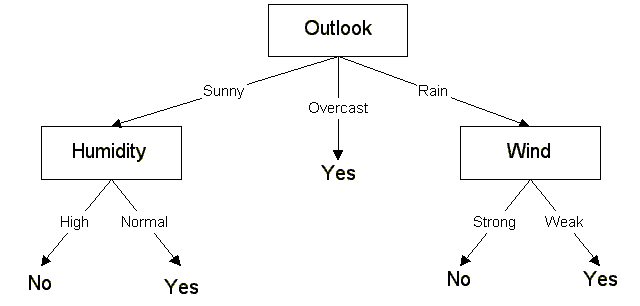
\includegraphics[width=1\textwidth]{Figures/dt.png}
  \caption{Example Decision Tree to predict if some students will play football.}
  \label{fig:dt}
\end{figure}

The most common algorithms to build decision trees are Quinlan’s ID3 \cite{Quinlan1986}, C4.5
 \cite{Quinlan1993} that came improve on ID3, and Breiman \& et al.’s Classification And 
 Regression Trees (CART) \cite{Breiman1984}.
 
 In the current work on prognosis,\hl[red]{ as seen in \ref{chapter:rw}}, the use of C5.0 is also found. C5.0 is an extension of C4.5 that, among several issues, presents a considerable performance optimization. 
 
Decision Trees result in a very easily understandable, like Figure \ref{fig:dt}, it is easy to see that some initial variable divides the data into two categories and then other variables split the resulting child groups. This information is very useful to the researcher who is trying to understand the underlying nature of the data being analyzed.

\subsection{Artificial Neural Networks \& Support Vector Machines}
\label{subsection:nn}

Artificial Neural Networks are computational models that approximate the functioning of the brain, in the sense that they are highly
 complex and non-linear. These networks are composed by a group of interconnected nodes, also called neurons, and are used for classification. 
 They have an input layer with nodes that correspond to data features, a various number of hidden layers and an output layer where the outcome 
 is represented as seen in Figure \ref{fig:nn}.

Contrarily to decision trees, neural networks do not present an easily-understandable model.
A neural network is more of a “black box” that delivers results without an explanation of how the results were derived. Thus, it is difficult or
 impossible to explain how decisions were made based on the output of the network.

\begin{figure}[!htb]
  \centering
  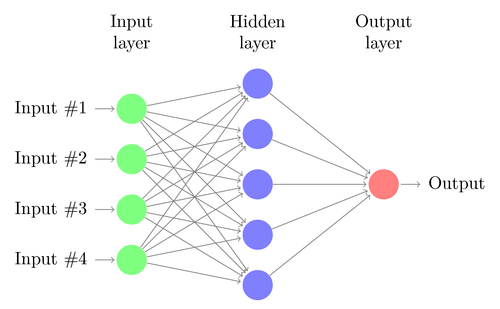
\includegraphics[width=1\textwidth]{Figures/nn.png}
  \caption{Artificial Neural Network structure.}
  \label{fig:nn}
\end{figure}

SVMs are another supervised machine learning technique, where a hyperplane is found that correctly separates the spatial representation of the data into the various classes.  For example, if the data is 2 dimensional, the hyperplane is a line that correctly divides the data and has the largest margin between itself and a data point, as seen in Figure \ref{fig:svm}. 

SVMs have been used with high accuracy and can with the right kernel can have good results even if the data is not linearly separable in the base feature space. They are memory intensive and require a lot of tunning and configuration.

 %\hl[red]{High accuracy, nice theoretical guarantees regarding overfitting, and with an appropriate kernel they can work well even if you're data isn't linearly separable in the base feature space. Especially popular in text classification problems where very high-dimensional spaces are the norm. Memory-intensive and kind of annoying to run and tune, though, so I think random forests are starting to steal the crown.}

\begin{figure}[!htb]
  \centering
  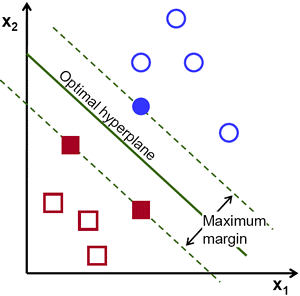
\includegraphics[width=0.75\textwidth]{Figures/svm.png}
  \caption{Example of 2D SVM optimal hyperplane.}
  \label{fig:svm}
\end{figure}

\subsection{Bayesian Classifiers}
\label{subsection:bc}

Bayesian classifiers are probabilistic classifiers that get their name by making use of the Bayes Rule of Inference. 

Naïve Bayes Classifier calculates the probability of a certain outcome class by considering that all features are independent,
 in other words by seeing how their value alone influences the outcome class. 

If the NB conditional independence assumption actually holds, a Naive Bayes classifier will converge quicker than
 discriminative models like logistic regression, so less data would be necessary.

\subsubsection{Bayesian Networks}
\label{subsubsection:bn}	

Bayesian networks are probabilistic graphical models, represented as directed acyclic graphs, where nodes represent random 
variables and edges the probabilistic dependency between them. These dependencies between variables are found using the theory of information.
% CHECK FACTS!!! \hl[red]{using statistical methods}\hl[blue]{nao +e bem assim! teoria da informaçao}. 

\hl[red]{Exemplo}

HMMs or Hidden Markov Models can be viewed as a specific case of the more general dynamic graphical models, where particular dependencies are assumed. Thus, HMMs and their variants can be interpreted as examples of DBNs.
An HMM is a stochastic finite automaton, where each state generates (emits) an observation. An HMM is described by a quintuple, ${N , M , A , B , \pi}$ where this symbols mean:

\begin{description}
	\item[$N$] = number of states in the model
	\item[$M$] = number of distinct observation symbols per state (observation symbols correspond to the physical output of the system being modelled)
	\item[$T$] = length of observation sequence
	\item[$O$] = observation sequence, i.e. , $O_1,O_2,…,O_T$
	\item[$Q$]  = state sequence $q_1,q_2,…,q_T$ in the Markov model
	\item[$A$] = ${a_{ij}}$ transition matrix, where $a_{ij}$ represents the transition probability from state $i$ to state $j$
	\item[$B$] = ${b_j (O_t)}$ observation emission matrix, where $b_j (O_t)$ represent the probability of observing $O_t$ at state $j$
	\item[$\pi$] = ${\pi_i}$ the prior probability, where $\pi_i$ represent the probability of being in state $i$ at the beginning of the
	experiment, i.e., at time $t=1$
	\item[$\lambda$] = $(A,B,\pi)$ the overall HMM model.
\end{description}

As mentioned above the HMM is characterized by $N, M, A, B$ and $\pi$. The $a_{ij}, b_i (O_t)$, and $\pi_i$ have the properties:

$ \Sigma_j a_{ij} = 1, \Sigma_t  b_i (O_t) = 1, \Sigma_i \pi_i = 1$ and  $a_{ij}, b_i (O_t)$, and $\pi_i >= 0$ for all $i,j,t$.


\subsection{Regression Analysis}
\label{subsection:regression}

Regression analysis is the use of a statistical analysis method used to measure the relation between variables. In other words, it helps to
 understand how a dependent variable varies with changes in one of the independent variables. 

Linear Regression is an example of regression analysis where a linear function is used to model the data. When the outcome variable,
 the dependent variable is binary or categorical, linear regression cannot be applied. In those cases it is used logistic regression.

 However, linear regression is appropriate only if the data can be modeled by a straight line function, which is often not 
the case.

Logistic Regression is a generalization of linear regression that, as just mentioned, is used to predict binary or categorical dependent
 variables. In this regression instead of predicting the estimate value of an event it predicts the probability of it occurring.

Regressions have comprehensible probabilistic interpretation and you can easily update your model to take in new data, unlike decision trees or SVMs. You can use this if you expect to receive more training data in the future that you want to be able to quickly incorporate into your model.

Another example of regression analysis that is also used in the healthcare domain is called Cox Proportional Hazard Models, which are a type
 of survival models, where the time to the occurrence of an event is related with one or more covariates that may be responsible. They show the 
 influence of variables in the time to an event occurrence.

In medical studies Cox Proportional hazard models are the most common method used for survival outcomes.

It is an extension of the logistic model to the survival setting. Similar to conditional logistic regression with conditioning only at time of 
events. In the logistic method we us a linear predictor while in the COX mode a hazard function is used. The hazard function dictates the risk of
 the outcome during the follow up time.
 
 \begin{equation}
  {\cal \lambda}(t|X) = {\cal \lambda}(t)e^{\beta X}
\label{eq:hazardFuntion}
\end{equation}

Where \( \lambda(t) \) is the hazard at time \(t\), and is usually estimated at the mean values of the predictors and \( \beta X\) is the linear predictor, 
\( \beta_1 \times x_1 + \beta_2 \times x_2 + ... + \beta_p \times x_p\)

 The linear predictor is usually centered at the mean value of the predictors, and \( e^\beta X \) then indicates the hazard
 ratio compared to the average risk profile.

\cleardoublepage % add new .tex files for new chapters

\chapter{Status of Affairs}
\label{chapter:rw}

In this chapter it will be overviewed the work that has been done in the area of automatic prognostic and diagnostic. Diagnostic because,
 even though this thesis will be about prognosis, it is said in \cite{Hendriksen2013} that the development, 
 validation and impact assessment of both cases can be mutatis mutandis applied. 

The prediction classification can be a diagnostic or a prognostic depending only on the amount of time until the outcome assessment. 
Being the options between the outcome assessment the present or the future, the former is a diagnostic and the latter a prognosis.

In the field of diagnosis the techniques used revolve around the same as in prognosis. Mainly it uses decision trees, artificial 
neural networks, association rules and Bayes classifiers as well as Support Vector Machines \cite{Kharya2012}.

There are three types of prediction that can be done when talking about prognosis:
\begin{itemize}
\item We can try to predict the probability of developing a disease or a state of that disease, in other words we can perform
 a risk assessment or predict the disease susceptibility;
\item We can predict if there will be recurrence of an event, for example if a cancer will recur after it was excised;
\item We can predict if the patient will be alive at a certain time point, known as \emph{survivability}. 

\end{itemize}

We will separate the review on prognostic prediction by disease in order to allow the comparison between the work being done in the various 
diseases. Showing that even though the same techniques are used they require different preprocessing and the end results are very data dependent.

We can find work on prognostic prediction as far back as 1980 \cite{Nash1980} where a regression analysis is used 
to find the predictive power of 17 features when predicting the survival of breast cancer patients. Also in the early
 90s \cite{Hanson1993} where logistic regression is used to predict Survival of HIV infected patients and
 \cite{Mangasarian1995} where dynamic programming is used to predict the time to recurrence of an excised cancer.
 
 \section{Alzheimer}
 \label{section:alz}
 
The Alzheimer’s disease (AD) is the most common form of dementia. It causes problems with memory, thinking and behaviour. 
Symptoms usually develop slowly and get worse over time, becoming severe enough to interfere with daily tasks and eventually 
leading to death. In order to predict the progress of the disease several techniques have been applied.

Alzheimer’s disease is associated with variable but shortened life expectancy, even at relatively early stages. For that
 reason having a survivability expectancy might be important for the patients and their carers to understand and plan ahead. 

In \cite{Paradise2009} they used Cox proportional hazards regression modelling for univariate and multivariate statistics. 

On the multivariate analysis in order to find the most predictive features a forward stepwise approach was used followed
 by a backward stepwise linear regression in order to confirm if the results were robust. 

The final model, SAM (Survival in Alzheimer’s Model) is a 4 point risk scale according to whether a patient has or not the
 identified risk factors (increasing age, Constructional praxis, Gait apraxia). A patient with two risk factors will have 
 an 80\% chance of surviving 12 months, but less than 50\% chance of surviving 3.5 years.

This study has some limitations like the fact that one of the features where it was built upon, was clinically obtained, by a
 standardized assessment by the same doctor. Also this model’s generalizability may be limited because the cohort was a convenience
 sample and was not recruited to be representative of the larger population of people with AD.

In \cite{Zhou2011}, Zhou et al. develop a new multi-task learning formulation based on the temporal group Lasso regularizer,
 in order to predict the Alzheimer’s disease progression, based on the Mini Mental State Examination (MMSE) and Alzheimer’s disease 
 Assessment Scale cognitive subscale (ADAS-Cog) scores, that give the cognitive status of a patient. The multi-task regression
 approach captures the relation of the task, and the regularizer ensures that a small set of features is used for the regression
 and that a large deviation between successive time points is penalized.

  \section{Cancer}
 \label{section:cancer}
 
Cancer, known medically as a malignant neoplasm, is a class of diseases characterized by out-of-control 
cell growth. It becomes harmful when faulted cells grow into lumps of tissue that are called tumors. The
 cancer may also end up by spreading when cancerous cells move through the lymphatic system or bloodstream.

Cancer is seen as a deadly disease, as most people end up dying from the cancer or its treatment. The ones 
that actually survive have twice the probability of developing a second cancer than the people that were never
 diagnosed with cancer. \cite{Rheingold2000}

Because of this the three types of prognosis are found in cancer research: there is the prediction of the
 probability of developing cancer, in other words we can perform a risk assessment or predict the cancer susceptibility,
 the prediction if there will be recurrence in the cancer after if it excised or the prediction if the patient will 
 be alive at a certain time point. 

In these three areas of prognosis we have the following work.

To perform the prediction of survival at 5, 10 and 15 years after the diagnostic, \cite{Lundin1999} uses artificial
 neural networks and logistic regression, showing that neural networks are consistent with logistic regression as is 
 represented in \ref{fig:LRvsNN}. 

 \begin{figure}[!htb]
  \centering
  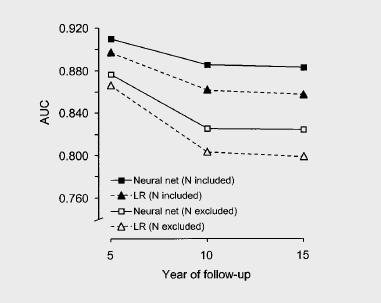
\includegraphics[width=0.75\textwidth]{Figures/LRvsNN.png}
  \caption{AUCs for the neural network and logistic regression (LR)}
  \label{fig:LRvsNN}
\end{figure}

In \cite{Steyerberg2005}, in order to decide which treatment is better for the patients’ well-being, a COX regression analysis
 is used to predict a score based on the regression coefficients, which classifies the patients in 3 different groups: the ones
 with good, intermediate or bad prognosis in terms of survivability. Using this knowledge of the degree of prognosis in addition
 with the short-term versus long-term benefits of each treatment, a better choice can be performed helping to improve the patient’s quality of life. 

To predict the overall survivability, at 1 year and 5 years mark, of patients with Acute Myeloid Leukemia, Breems et al. applied 
multivariate Cox regression analysis with stepwise backward selection on the patient’s age at the time of the relapse, length of relapse 
free interval, previous stem cell transplant and cytogenetics. 

Like in \cite{Steyerberg2005}, they used the regression coefficients has a score function that is used to classify the patients \cite{Breems2005}

The purpose of \cite{Delen2005} is to develop predictive models and discover/explain relationships between certain independent variables and the
 survivability, 5 years after the diagnosis, in the context of breast cancer. Delen et al. per-form a comparative study with decision trees (C5.0),
 MLP neural network and logistic regression. Showing that with the SEER dataset and using a tenfold cross validation, the decision tree performed 
 the best out of the three with accuracy of 0.9362, closely followed by the neural network that achieved 0.9121 and the logistic regression that
 got 0.8920.

In the presence of microarray data, the clinical data is usually underused say Gevaert et al. that in \cite{Gevaert2006} propose the usage of Bayesian 
networks to equally use both sources of data and that way get better results when performing the prognosis. 

They evaluated three methods for integrating clinical and microarray data: decision integration, partial integration and full integration 
and used them to classify publicly available data on breast cancer patients into a poor and a good prognosis group. The partial integration
 method is most promising and has an independent test set area under the ROC curve of 0.845.

In the problem addressed in \cite{Anagnostopoulos2006}, a neural network calculates a time interval that corresponds to a possible right
 end-point of the patient’s disease-free survival time, in other words it predicts the time to recur (TTR) by classifying the patient into 
 4 classes, TTR $\leq$ 1 year, TTR $\leq$ 3 years, TTR $\leq$ 6 years and TTR $>$ 6 years. The accuracy of the neural network was measured through a
 stratified tenfold cross validation approach. Sensitivity ranged between 80.5 and 91.8\%, while specificity ranged between 91.9 and 97.9\%,
 depending on the tested fold and the partition of the predicted period. 

In \cite{Bellaachia2006} a comparison is made between different data mining techniques, Naïve Bayes, Neural Networks and Decision Trees 
when predicting survivability of breast cancer patients 5 years after the diagnose. For that comparison the Weka toolkit and the SEER 
Dataset is used, which is composed by demographic data (age, race, etc.) and clinical data (Extension of tumor, stage of cancer, etc.). 
After the tests the conclusion was that both, decision trees and neural networks, had better and similar performance with accuracy around 86\%, 
though in the computational time the approaches did differ where the neural networks model took 12 times more to be built.

Because of the neural networks’ ability to consider variable relations and create non-linear predictions models they are a very used 
method for cancer survivability prediction, how long after surgery it is expected that the cancer will recur. Here in \cite{Chi2007} it 
is shown that they can be used to predict the probability of survivability, and based on a threshold classify them as good or bad prognosis,
 with 2 different datasets. 

 \cite{Endo2008} uses Logistic Regression model, Artificial Neural Network (ANN), Naive Bayes, Bayes Net, Decision trees with naïve Bayes,
 Decision Trees (ID3) and Decision Trees (J48) to predict breast cancer survival at 5 years learning that Logistic regression has the 
 highest accuracy along with J48. Decision trees tend to have high sensitivity. But is also shown that the best algorithm depends on the object
 and the dataset.

Because there is no use of fuzzy logic when performing cancer prognosis, most of the current work uses neural networks that yield difficult
 to understand models and that there is no use of hybridization of machine learning techniques, Muhammad Umer Khan et al. investigated a hybrid
 scheme based on fuzzy logic and decision trees on the SEER dataset. They performed experiments using different combinations of number of 
 decision tree rules, types of fuzzy membership functions and inference techniques in order to predict the patient survivability. They end up
 by comparing the performance of each for cancer prognosis and found hybrid fuzzy decision tree classification is more robust and balanced
 than the independently applied crisp classification. \cite{Khan2008}

In \cite{Delen2009}, Delen uses a handful of data mining techniques, decision trees, artificial neural networks and sup-port vector machines
 along with the most common statistical analysis tool, logistic regression, to build a prediction model for prostate cancer survivability and 
 comparing their performance. The results indicated that SVMs are the best predictor with a test data set accuracy of 92.85\%, followed by ANNs 
 with an accuracy of 91.07\%, followed by decision trees with an accuracy of 90.00\% and logistic regression with an accuracy of 89.61\%.

Jong Pill Choi et al. compared the performance of an Artificial Neural Network, a Bayesian Network and a Hybrid Network used to predict breast
 cancer prognosis. The hybrid Network was a combination of ANN and Bayesian Network. All the techniques were used on nine variables of the
 SEER data that were clinically accepted. In this research the accuracy of ANN (88.8%) and Hybrid Network (87.2%) were very similar and they
 both performed much better than the Bayesian Network. \cite{Choi2009}

In \cite{Sun2011} improve the L1-L2 norm SVM that has automatic feature selection for prognostic prediction to use regression, and developed
 the algorithm to utilize the information of censored data. The proposed method is compared with other seven prognostic prediction methods,
 namely CART, MARS, RSA, RRLC, L1-norm SVM, L2-norm SVM, Elastic Net, penalized Buckley-James, on three real world data sets. The experimental 
 results show that the proposed method performs consistently better than the medium performance and that it is more efficient than other
 algorithms that achieved similar performance.

Kharya performs a review of use cases where data mining has been used to per-form prognosis of cancer disease. It shows that the most 
common cases, while they may need to be tested on larger set of examples in order to find rules with higher level of statistical confidence, 
they do find statistically significant associations that can help predict a patients’ future. In this study they show examples using decision
 trees, neural networks, logistic regression as well as Bayesian networks. \cite{Kharya2012}

In \cite{Wang2012}, the prediction of survivability on the 5 year mark after diagnose were performed using decision trees and logistic regression.
 Using the SEER dataset Wang et al. show that logistic regression, even though the accuracy is similar, outperforms decision trees by having a
 higher g-mean and by comparing the ROC curve and AUC.

In \cite{Saxena2013} instead of using the complete Wisconsin Prognostic Breast Cancer data set, a pre-processing technique 
is used in order to reduce the number of features and improve the accuracy of polynomial neural network that was later used. 
The pre-processing technique is called principal component analysis (PCA) and it is a statistical procedure that returns a set
 of principal components. These principal components are less than or equal to the number of original features and they are ordered 
 by their importance in the variability of the outcome. It is shown that the use of PCA is preferred to normalization, having the 
 former more accurate results.

Using the SEER database Lakshmi et al. perform a comparison of a number of techniques when diagnosing and predicting 5-year
 survivability of patients diagnosed with breast cancer. The techniques that were compared were: C4.5, SVM, PNN, k-NN, Binary 
 Logistic Regression as well as Multinomial Logistic Regression, Partial Least Squares Regression (PLS-DA), Partial Least Squares 
 Linear Discriminant Analysis (PLS-LDA), k-means and Apriori Algorithm. In the end this study shows that PLS-DA performs the best
 with lowest computation time and highest accuracy. \cite{Lakshmi2013}

\section{Diabetes}
\label{section:diabetes}

Diabetes, often referred to by doctors as diabetes mellitus, describes a group of metabolic diseases in which the person 
has high blood glucose (blood sugar), either because insulin production by the pancreas is inadequate, or because the body's
 cells do not respond properly to insulin, or both.

There are three types of diabetes: type 1 is when the body does not produce insulin, type 2 is when the body does not 
produce enough for normal function or the cells in the body do not react to insulin, insulin resistance and the third type 
affects females when pregnant. They develop high levels of blood sugar and don’t have enough insulin to transport it. 

In \cite{Lindstrom2003} a risk score to predict the incidence of diabetes was developed. The multivariate logistic regression model
 coefficients were used to assign each variable category a score. The Diabetes Risk Score was composed as the sum of these individual
 scores. In the final predictive model there were 7 features selected, Age, BMI, waist circumference, history of antihypertensive
 drug treatment and high blood glucose, physical activity, and daily consumption of fruits, berries, or vegetables. 

The model was developed using a cohort study from 1987 and another from 1992 where the subjects received by mail a questionnaire 
on medical history and health behavior and an invitation to a clinical examination.

The score that was derived from the regression coefficients ranged from 0 to 20 and the value $\geq$ 9 was able to predict diabetes
 with a sensitivity of 0.78 and 0.81, specificity of 0.77 and 0.76 in the 1987 and 1992 cohorts, respectively.

In order to improve the work of Lindström et al. the author of \cite{Balkau2008} aims to describe sex-specific lifestyle and clinical
 diabetes risk factors in a French population followed over 9 years in order to aid in identifying those at risk for incident diabetes.
 The data is composed by clinical along with biological data that was gathered every 3 years over a period of 9 years. In this study 
 patients with al-ready incident diabetes in the beginning were excluded as well as the patients with unknown status of diabetes at 
 the end. The author performed a statistical analysis over the data in order to find the most predictive features. Balkau et al. used 
 logistic model to test for interactions with sex, Parsimonious logistic regression models were selected using forwards and backwards
 as well best model selection criteria using all parameters; the Hosmer-Lemeshow goodness-of-fit test was the principal criteria for
 selection of a model. 

The resulting models, clinical and clinical + biological, were able to predict the incidence of diabetes over the 9 year period.
  They studied the influence of gender in the model, learning that the predictive functions were different for each sex. 

Because the currently available screening tools for identifying individuals at high risk of type 2 diabetes can be invasive,
 costly and time consuming Xie et al. devel-oped a tool to identify individuals in the Chinese general population with high risk
 of developing type 2 diabetes (Xie, et al., 2010). Using data from 994 persons with type 2 diabetes and 13 129 persons with normal
 fasting glucose, test performed to find diabetic patients, aged 35-74 years. After a Classification and regression tree (CART)
 analysis, performed separately in men and women, two risk trees were obtained: one with 5 risk levels for men, and another with 
 8 for women. Being that women with a diabetes risk level (DRL) of 8 and men with a DRL of 5 are at the highest risk of type 2 
 diabetes. The CART results were compared with multivariable logistic regression model including the same predictors achieving 
 both the same AUC of 0.71 vs. 0.73 in women and 0.65 vs. 0.69 in men, in the training and testing samples, indicating a good 
 prediction above chance.

In \cite{Chen2010} a risk score is built for the prediction of type 2 diabetes in a 5 year follow up study between 1999 and
 2004, using demographic data, like age, sex and ethnicity, some feature that represent the history of the patient and clinical
 tests. The score was built using a logistic regression analysis where the features’ coefficients were rounded up and used as
 a score if that feature was present. It was found that this diabetes risk score was a useful non-evasive method to identify
 Australian adults at high risk of type 2 diabetes who might benefit from interventions to prevent or delay its onset.

\section{Venous Thromboembolism}
\label{section:venous}

Venous Thrombosis is a blood clot that forms within a vein. A common cause of venous thrombosis is the deep vein thrombosis that can turn into a pulmonary
 embolism, which can be lethal. Venous thromboembolism is a disease that includes both deep vein thrombosis (DVT) and pulmonary embolism (PE). 

In order to predict the outcome in a 30-day period of patients that had a pulmonary embolism, Aujesky et al. used clinical variables 
that were shown to be related with the death of patients with PE. These variables included demographics, comorbid conditions, physical
 examination findings, and laboratory and chest x-ray findings. On that data a stepwise logistic regression analysis was performed to
 create the pre-diction rules that classify within 5 levels of mortality risk. \cite{Aujesky2005} 

\cite{Eichinger2010} Based on a cohort study of 929 patients that had a first unprovoked deep vein thrombosis, Eichinger et al. perform 
a COX hazard proportional analysis to learn the relevance of, previously selected, clinical and laboratorial data in the recurrence of the
 thrombosis. Using those values a nomogram was created that can give risk probability of recurrence and correctly classify patients in risk categories. 

The risk of recurrence in a patient that had an unprovoked thromboembolism is between 5 and 7\% in the first year, that risk can be
 significantly reduced by the ad-ministration of oral anticoagulation therapy. On the other hand, the risk of major bleeding with ongoing 
 oral anticoagulation therapy among venous thromboembolism patients is 0.9–3.0\% per year with an estimated case-fatality rate of 13\%.
 Given that the long-term risk of fatal hemorrhage appears to balance the risk of fatal recurrent pulmonary embolism among patients
 with an unprovoked venous thromboembolism, clinicians are unsure if continuing oral anticoagulation therapy beyond 6 months is
 necessary. In \cite{Rodger2008}, Rodgers et al. used conditional logistic regression with forward variable selection, they conducted
 multivariable analysis with recurrent venous thromboembolism as the dependent variable in order to develop a risk score that may help
 clinicians decide whether to stop the anticoagulation therapy or not. 

They concluded that it may be safe for women who have taken oral anticoagulants for 5–7 months after an unprovoked venous thromboembolism 
to discontinue therapy if they have 0 or 1 of the following signs or symptoms: hyperpigmentation, edema or redness of either leg;
 a D-dimer level of 250 $\mu/L$ or more while taking warfarin; BMI 30 $kg/m2$ or more; and age 65 years or more.
 A decision rule for mean was not able to be found.

In cite{Tosetto2012} another risk prediction score is develop for the same task as \cite{Rodger2008}, to help clinicians know if the anticoagulant
 therapy may stop, in this case after an initial period of at least 3 months.

The score (DASH, D-dimer, Age, Sex, Hormonal therapy) was developed firstly by identifying variables highly correlated with the recurrence by using
 COX regression. In the initial full model there were 7 features: D-dimer; age; patient sex; hormone use at time of VTE (in women); mode of initial
 presentation (DVT alone or DVT and PE); and previous history of cancer, not active at the time of initial event. At first, the model was reduced 
 using backward selection of features, but because this may lead to an overly optimistic model they evaluated the degree of over-optimism both 
 by a heuristic formula and by linear shrinkage with bootstrapping, this means that they adjust the regression coefficient based on the calculated optimism. 

In the end, by multiplying the corrected coefficient by a common value and rounding to the nearest integer the score was found. The annualized 
recurrence risk was 3.1\% for a score $\leq$ 1, 6.4\% for a score $=$ 2 and 12.3\% for a score $\geq$ 3. By considering at low recurrence risk those
 patients with a score $\leq$ 1, life-long anticoagulation might be avoided in about half of patients with unprovoked VTE.

 \section{HIV/AIDS}
 \label{section:hiv}
 
 Human immunodeficiency virus/ acquired immunodeficiency syndrome (HIV/AIDS) is a disease that affects the human immune system when infected with
 HIV. Acquired Immunodeficiency Syndrome is the final stage of HIV infection. People at this stage of HIV disease have badly damaged immune
 systems, which put them at risk for opportunistic infections that may lead to death.

In terms of prognosis of HIV/AIDS, it usually refers to the likely outcome of HIV/AIDS. It may also include the duration of HIV/AIDS, 
chances of complications of HIV/AIDS, probable outcomes, prospects for recovery, recovery period for HIV/AIDS, survival rates, death rates,
 and other outcome possibilities in the overall prognosis of HIV/AIDS. 

The ART Cohort Collaboration is an association between 13 cohort studies from Europe and North America, it gathers data from patients who
 are infected with HIV-1 and started highly active antiretroviral therapy (HAART). In \cite{Egger2002}, Egger et al. build a prognostic
 model to predict the development into AIDS or death and to death alone. The prognostic models were parametric survival models based on the 
 Weibull, loglogistic, and lognormal distributions showing that the Weibull was the one that generalized best stratified by baseline CD4 cell
 count and transmission group (sexual contact, drug injection, etc.).

Using an adaptive fuzzy regression technique, Don et al. predicted the length of survival of AIDS patients based on their CD4, CD8 and 
viral load counts. A comparison was made with fuzzy neural networks getting both the techniques similar results. The accuracy of the 
prognosis ranged between 60 and 100\% depending on what year was being predicted. \cite{Dom2009}

With data from patients diagnosed with AIDS between 1987 and 2007 from the University Hospital of Kuala Lumpur. Abdul-Kareem et al. 
developed a Classification And Regression Tree (CART), based on clinical and demographic data, to predict survival of patients during
 that interval. The author managed to get an accuracy between 60-93\% depending on the year that’s being predicted.
 \cite{AbdulKareem2010}

 \section{Kidney Failure}
 \label{section:kidney}
 
Kidney failure, also called renal failure or renal insufficiency, is a medical condition in which the kidneys fail to adequately filter waste
 products from the blood. There are 5 stages of kidney failure, being the first mildly diminished renal function, stage 2 and 3 need more 
 level of care from the physician in order to deal with the dysfunction, stages 4 and 5 require the patients to endure in active treatment
 in order to survive. This active treatment may come in the form of dialysis or kidney transplant. 

Due to the enormous amount of people in kidney transplantation waiting list Ahn et al. try to predict, in \cite{Ahn2000}, the 
one year survival of patients with kidney transplantation in order to make a more informed decision when choosing a patient for 
transplant. For that they built a Bayesian Network on 35,366 kidney transplants performed in the United States between 1987 and 1991.

For the same task, in \cite{Petrovsky2002}, are reported the results of training an ANN, that was able to correctly predict 84.95\% 
of successful transplants and 71.7\% of unsuccessful transplants.

Later, in \cite{Shadabi2004}, Shadabi et al. try to improve on Petrovsky’s work. For this Shadabi et al. used
 artificial neural networks instead of the more usually used statistical techniques that don’t provide enough information for complex
 problems. They tried to improve on Petrovsky and et al.’s work by using a radial basis function network and prediction of the outcome
 at the 2 years mark. The accuracy of this approach was very similar, when used on the same data set, to the one proposed in 
 \cite{Petrovsky2002} and despite the use of a range of pre-processing and ANN solutions for prediction of outcomes of 
 kidney transplants, they found that the resultant accuracy of approximately 62\% was probably too low to be of any clinical use. 

Like the previous papers \cite{Shadabi2004}, etc. in \cite{Osofisan2011} artificial 
neural networks are used, on data monitored when providing kidney dialysis treatment, to determine the features are related with
 patients’ life expectancy as well as detect the existence of renal failure. It provides a model that can help and support a better 
 understanding of a patient’s evaluation results.

Kusiak et al. \cite{Kusiak2005} used rough sets and decision trees to predict the survival time of patients undergoing
 kidney dialysis. Although they had a limited dataset and the lack of many important variables they show the potential for making 
 accurate decisions for individual patients is enormous and the classification accuracy is high enough (above 75–85\%) to warrant the
 use of additional resources and further research.

Wolfe et al. \cite{Wolfe2008} use Cox regression analysis to calculate the LYFT score (life years from transplant), in order
 to develop a novel kidney allocation system based on this prediction of lifespan. The LYFT score was higher for younger patients and 
 smaller for diabetic patients.

Li et al. \cite{Li2010} present the development of a Bayesian belief network classifier for prediction of graft status and 
survival period in renal transplantation using the patient profile information prior to the transplantation. They developed two
 classifiers one to predict the status of the graft and another to predict its survival period. While the first one achieved a prediction
 accuracy of 97.8\% and true positive values of 0.967 and 0.988 for the living and failed classes the second model showed only 68\% accuracy.
 
 \subsection{Organ Failure}
 \label{subsection:organ}
 
 Prognosis work that is not about kidney failure can also be found. In \cite{Oztekin2009} a study is performed where the authors
 used neural networks, decision trees as well as logistic regression, when trying to predict a patients’ survival after a combined heart-lung
 transplant. The predictive models’ performance in terms of 10-fold cross-validation accuracy rates for two multi-imputed datasets ranged 
 from 79\% to 86\% for neural networks, from 78\% to 86\% for logistic regression, and from 71\% to 79\% for decision trees.

Also, survival analysis of liver transplant patients in Canada was done by Hong et al. \cite{Hong2006} here they apply Cox proportional 
hazards analysis to evaluate many clinical and physical parameters’ relation to the survival of the patient. A drawback of that study is that
 they use a very limited set of variables.

Again in liver transplant there is this study \cite{Ataide2012}, where the Kaplan–Meier method and Cox regression are used to evaluate
 the relevance of the up-to-seven criteria, with 7 being the sum of the size and number of tumors for any given hepatocellular carcinoma (HCC),
 when predicting the survival of patients with hepatocellular carcinoma that perform liver transplant. 

 \section{Critical Analysis}
 \label{section:analysis}
 
 What we can see from the status of automated prognosis in the various diseases presented above, is that nowadays it is made without 
 contemplating any temporal information. And it is our opinion that using it may considerably improve the results achieved, since it
 will mimic physicians’ procedures. 

None of the previously presented approaches takes advantage of the evolution of a patient in order to increase its’ prognostic
 accuracy and when it is used it is in some sort of feature that represents this evolution. The time, as a dimension, is being 
 over-looked when building a prognostic model and it should be included in the process.

Another disadvantage of the work that has been done is that its’ results are very data dependent. \cite{Endo2008}
 shows that there is no best technique to perform overall prognosis and that the result of a technique depends highly on the data 
 being used. In other words there is no general solution that can be used in more than one dataset maintaining their performance.

Another problem that is notable in this review of prognosis work is that there is no evolution or search for improvement with
 only a few of the papers being based and working on improving some earlier work. There is a worry to develop new prediction 
 models before validating the already existing ones.
 
 \subsection{Difficulties in using classification for prognosis}
 \label{subsection:difficulties}
 
One of the major setbacks when trying to perform prognosis, is the fact that the data is, what is called, censored. This means that 
the value of a feature of the data is only partially known. In our case this feature is the outcome, where, for example, when 
predicting cancer recurrence we know the value if the cancer has recurred while on the other case, we can’t say with certainty 
that it won’t recur, just the amount of time that has passed since the cancer was removed. 

This introduces a level of uncertainty in data that needs to be handled by the data mining technique to be used.

Other difficulty when performing prognosis using classification is finding the correct dataset to train the model. The data
 should be from a cohort study, what enables better measurements of the features and helps to keep track on the outcome.

Also given the characteristics of the task in hand, difference between patients, using one predictor (or feature) is rarely 
descriptive enough to help. Doctor’s use a various amount of features about patients to be able to give a prognosis and so 
also needs to happen when performing the prognosis computationally. A multivariable approach should be used in order to take
 into account the relations between features when developing the best prognostic model.

Features, also called predictors, can be data from the patient’s demographic (age, gender, etc.), clinical history, physical 
tests, and disease characteristics. They should be well defined and, so they could be used in real clinical situations.



 
\cleardoublepage % add new .tex files for new chapters

\chapter{Approach}
\label{chapter:approach}

Classification is the problem of determining to which of a group of categories an observation belongs to. 
Formally you can represent the classification problem as finding the correct class $y$  using the observation
 features $\bar{x}$ in the pair $(\bar{x},y)$, where $\bar{x}$ is the feature vector and $y$ the class.

\begin{equation}
	\bar{x} = < x_1,x_2,...,x_n >
\label{eq:featurevector}
\end{equation}
 
 Applied to the diagnosis/prognosis problem this is what is currently being done, where a model is created to discover
 $y_n$  from $\bar{x}_n$. As already mentioned the difference between a prognostic model and a diagnostic model is just the
 time between the present and the supposed time of $y_n$. 

That is why we are introducing time, the addition of time to the equation turns the pair $(\bar{x},y)$ into the triplet
 $(\bar{x}_i,y_i,t_i )$ where $t_i$ is a timestamp, $\bar{x}_i$ the feature vector in at time $t_i$ and $y_i$ the class also at time $t_i$.

 \begin{equation}
	\bar{x}_i = < x_{i1},x_{i2},...,x_{im} >
\label{eq:temporalvector}
\end{equation}
 
 In this case we have a sequence S of triplets, that is ordered and that can be used to predict a whole new 
 triplet $(\bar{x}_{n+1},y_{n+1},t_{n+1})$.
 
  \begin{equation}
	S= (\bar{x}_1,y_1,t_1 )… (\bar{x}_n,y_n,t_n ) \Rightarrow (\bar{x}_{n+1},y_{n+1},t_{n+1} )
\label{eq:sequence}
\end{equation}

Supposing $t_{n+1}$ is known our objective is to find $y_{n+1}$, the class in a future point in time.

In order to find $y_{n+1}$ we propose the following approaches:
\begin{enumerate}
\item{ To only find $y_{n+1}$

In this approach $y_{n+1}$ is found just based on the values for the feature vector $\bar{x}$ at each point of time, ignoring the values of $x_{n+1}$
  and do not trying to estimate them.
\begin{equation}
	y_{n+1} = f(x_{i} :1 \leq i \leq n)
\label{eq:approach1}
\end{equation}
  }
\item{ To find $(\bar{x}_{n+1},y_{n+1})$
	
Here  $y_{n+1}$ is found using diagnostic model on the feature vector $\bar{x}_{n+1}$ that, itself is found using various approaches:
	\begin{enumerate}
		\item{ $x_{n+1,k}=f(\bar{x}_j:1\leq j \leq n)$
		\begin{enumerate}
			\item{We can determine $x_{n+1,k}$ using the past values from the same feature, $x_{1,k},..., x_{n,k}$ . }
			\item{We can determine $x_{n+1,k}$ using the past values from all the features $\bar{x}_{1,k},..., \bar{x}_{n,k}$ and $y_1,...,y_n$.}
		\end{enumerate}
		}
	\end{enumerate}
}
\end{enumerate}

In the approach $i.$, only the values of one feature are used to predict the value of that feature, i.e. in order to predict $x_{n+1,i}$ only 
the values $x_{1,i},..., x_{n,i}$ will be used. 

This approach will be performed by using and/or adapting the techniques used in time series prediction. Here we need to find the technique 
that best deals with data that might not be numeric. This approach does not take into account the complex nature between features. 

On the approach $ii.$, all the features and eventually also the class are used when predicting each feature value. This approach will be 
performed using core data mining techniques, like decision trees and SVM, which capture the dependence relations between features.

These two approaches, described above, will work as baseline for comparison with the rest of the work. Where one represents the use of 
time but lacks in capturing the intrinsic relation between features and another the opposite, while capturing the dependence relation 
between features misses in the explicit use of time.

Another approach is to develop a representation for $x_{1_k},...,x_{n_k}$ that captures its’ evolution. Using that new representation of the 
data we can develop a new model that uses the relation between features as well as temporal patterns to correctly classify $y_{n+1}$.

\section{example}
\label{section:example}

Let’s assume we have clinical and laboratorial data for a set of patients with Alzheimer’s disease. The data itself could be 
represented like in \ref{tab:diagnostic}. 

\begin{table}[h]
\begin{center}
\begin{tabular}{ccccccc}
\textbf{Patient ID} & \textbf{Gender} & \textbf{Age} & \textbf{HBP} & \textbf{LBP} & \textbf{Degree of Progression} & \textbf{Time Step} \\ \hline
25         & M      & 65  & 160 & 88  & 1                     & 0         \\
25         & M      & 65  & 140 & 90  & 1                     & 1         \\
25         & M      & 65  & 138 & 85  & 1                     & 2         \\
25         & M      & 65  & 134 & 81  & 1                     & 3         \\
25         & M      & 65  & 141 & 88  & 2                     & 4         \\ \hline
\end{tabular}
\caption{Table 1}
\label{tab:diagnostic}
\end{center}
\end{table}
 
As seen in \ref{tab:diagnostic} we have $N$ time steps of data, in this case 5, we are going to use those in order to perform prognosis. As described
 in the last section we have 2 approaches to doing that, in the first we only use the past values of a feature to predict the future
 value of that feature, that is, for example with the high blood pressure, we can use HBP in times $0,1,2,3,4$ in order to predict $5$, and
 the same for every other feature.

In \ref{tab:approach1} we can see the data what would be used in order to predict HBP at time $5$.

\begin{table}[h]
\begin{center}
\begin{tabular}{cccccc}
\textbf{HBP\_0} & \textbf{HBP\_1} & \textbf{HBP\_2} & \textbf{HBP\_3} & \textbf{HBP\_4} & \textbf{HBP\_5} \\ \hline
160             & 140             & 138             & 134             & 141             & ?					\\ \hline        
\end{tabular}
\caption{Table 2}
\label{tab:approach1}
\end{center}
\end{table} 

The second option we would use every feature value to predict each one. In this case we would use the time steps $0$ to $4$ of every feature, as can be seen in \ref{tab:approach2} to predict
 HBP $5$, as well as every other feature.
 
 \begin{table}[h]
 \begin{center}
\begin{tabular}{ccccccccccccc}
\textbf{Patient ID} & \textbf{Gender} & \textbf{Age\_0} & \textbf{HBP\_0} & \textbf{LBP\_0} & \textbf{Age\_1} & \textbf{HBP\_1} & \textbf{LBP\_1} & \textbf{…} & \textbf{Age\_4} & \textbf{HBP\_4} & \textbf{LBP\_4} & \textbf{HBP\_5} \\ \hline
25                  & M               & 65              & 160             & 88              & 65              & 140             & 90              &            & 65              & 141             & 88              & ?              \\ \hline
\end{tabular}
\caption{Table 3}
\label{tab:approach2}
\end{center}
\end{table}

At the end of this two approached the result is the same, which is a complete data row at time step 5.

Using that predicted data on a diagnostic model that was previously trained on data like in \ref{tab:diagnostic}.
 We would get the final Prognosis.
\cleardoublepage
 
\chapter{Approach2}
\label{chapter:approach2}


\hl{In the medical context, diagnosis is the use of patient’s data, demographic and clinical, in order to understand 
and classify the current health condition of a patient \cite{Steyerberg2005}. From a formal point of view, and in the computer-based 
context, let $A$ be a set of variables (either known as attributes) and $C$ a set of possible classes. Given an instance
 $\bar{x}_i$ described by a set of $m$ variables from $A$, say $\bar{x}_i = (x_{i,1},... ,x_{i,m})$, the goal is to discover the most
 probable value $y_i$, which corresponds to its class or status, with $y_i \in C$, as in \ref{eq:classification}.}

\begin{equation}
	\bar{x}_i = (x_{i,1},... ,x_{i,m}) \rightarrow y_i
\label{eq:classification}
\end{equation}


\hl{In a classification context, this is done in two steps: first by producing a classification model $M_D$, based on a set of known
 pairs $(x_i, y_i)$ – the training dataset, and second, by applying the discovered model to each instance to classify.}

\hl{On the other hand, \emph{prognosis} is the foreseeing or prediction of the risk or probability of a certain health event happening,
 in the future, using the clinical and non-clinical data. It is the medical prediction of how the pair patient disease is going
 to evolve in a specified period of time.}

\hl{To do this prognosis, a physician will use data that relates the patient to a certain part of the population, i.e. demographic data,
 as well as the patient’s and patient’s family clinical history. This means that the evolution of the patient is important in the
 prediction of his next state. Simply putting, if a patient is showing improvement in a certain factor that is responsible for
 some disease, it is more probable that his prognosis related to that disease is better than if it the patient had the same 
 value but that factor was deteriorating.}

\hl{As previously stated, in the process of making a prognosis a physician uses the medical history of a patient. This includes
 the different states a patient has been in the form of various clinical analyses he had done in different points over time.
 The need to use this sequential information shows the utmost importance that time has when predicting someone’s survivability,
 risk of recurrence.}

\hl{Considering all of this, then the prognosis task can be formalized as follows:}

\hl{Let a patient be represented by a sequence of pairs, $(\bar{x}_i^1,y_i^1 ),...,(\bar{x}_i^n,y_i^n )$ , then the goal is to predict
 his $y_i^{n+1}$ value – equation \ref{eq:goal1}. Note that the different values for $y_i^t$ may be observable (available) or non-observable 
 at time instant $t$ for instance $i$.}


\begin{equation}
	(\bar{x}_i^1,y_i^1 ),...,(\bar{x}_i^n,y_i^n ) \rightarrow y_i^{n+1}
\label{eq:goal1}
\end{equation}


The traditional classification approach has been applied to prognosis with modest success, as seen above. In all described 
cases, the evolution of single variables was not explored, and actually, the different time instances of their values were
 addressed separately, ignoring any possible hidden structure, in the majority of approaches. On the other hand, the analysis 
 of time series is applied to predict the next outcome of a single variable.

By recognizing that estimation may be used to fill unseen variable outcomes, which in turn may be used to improve classifiers
 accuracy, as in asap classifiers \cite{Antunes2010}, we propose to transform the prognosis into a diagnosis task, by estimating the values
 of the variables that constitute the snapshot in the future point in time.

Formally, let $A$ be a set of attributes, $C$ be a set of possible classes and $n$ be the number of observations. Let the $t^{th}$ observation,
 described by $m$ variables from $A$, be the pair given by $(\bar{x}_i^t,y_i^t)=(x_{i1}^t,...,x_{im}^t,y_i^t)$ that says that at observation $t$
 the instance is described by $x_i^t$ (the observable values) and classified as $y_i^t \in C$(the predicted value). Given an instance 
 described by an ordered set of $n$ observations, the goal is to predict the ${n+1}^{th}$ observation, as in equation \ref{eq:goal}.

\begin{equation}
	(\bar{x}_i^1,y_i^1 ),...,(\bar{x}_i^n,y_i^n ) \rightarrow y_i^{n+1}
\label{eq:goal}
\end{equation}

The difference to the definition \ref{eq:goal1} is the need to predict the entire ${n+1}^{th}$ observation, not only the predicted 
value $y_i^{n+1}$. Indeed, if there is a model $M_D$, that from observable values is able to determine the predicted value, it is 
enough to estimate the observable values in the ${n+1}^{th}$ observation, and from them to predict the predicted value. This model $M_D$ is
 just a simple diagnosis model as in equation \ref{eq:classification}.

 According to this formulation, a prognosis model, $M_P$, is then the composition of several models: one estimation model $M_{Ek}$ per each 
 observable variable $X_k$ and a diagnosis model $M_D$ able to predict the class given an observation, as in equation \ref{eq:prognosis}, where $n$ corresponds 
 to the number of available observations and $m$ the number of variables for describing each observation.

\begin{equation}
	M_P ((\bar{x}_i^1,y_i^1 )\space...\space(\bar{x}_i^n,y_i^n )) = M_D (M_{E1} (\bar{x}_i^1 \space...\space \bar{x}_i^n ) \space...\space M_{Em}
	(\bar{x}_i^1 \space...\space \bar{x}_i^n ))
\label{eq:prognosis}
\end{equation}

By transforming the prognosis problem into a diagnosis task, the challenge becomes to be able to estimate the observation in the
 time point to predict, which translates into the definition of the estimation models per each observable variable.

As stated above, the art of prognosis is based on the analysis of the evolution of the different variables along time. Therefore,
 estimation models should be able to recognize verified evolution trends in the estimation of future values. 

In this manner, we propose that an estimation model for a single variable $X_k$, say $M_{Ek}$ should be a function from a sequence of the
 observed values to an $X_k$ value. In particular, we propose two different approaches: the \emph{univariate-based} and 
 the \emph{multivariate-based estimations}.

A \emph{\underline{u}ni\underline{v}ariate-based model} for variable $X_k\space(UvE)$ is a function from a sequence of $n$
 values of $X_k$ to its next value, $x_k^{n+1}$, as
 in equation \ref{eq:uve}, where $Dom_{Xk}$ represents the domain of variable $X_k$. These models only explore the individual values of a 
 variable, ignoring any influence from other variables.
 
\begin{eqnarray}
	M_{UvEk}:[Dom_{Xk}]^n \rightarrow Dom_{Xk}        \\ \label{eq:uve}
	M_{UvEk}(x_k^1 \space...\space x_k^n) = x_k^{n+1} \nonumber
\end{eqnarray}

On the counterpart, a \emph{\underline{m}ulti\underline{v}ariate-based model} for variable $X_k \space (MvE)$ is a function from a sequence 
of $n$ vectors of $m$ variables, including $X_k$, to its next value, $x_k^{n+1}$ – see equation \ref{eq:mve}.

\begin{eqnarray}
	M_{MvEk}:[Dom_{X1} \times ... \times Dom_{Xm}]^n \rightarrow Dom_{Xk}  \\ \label{eq:mve}
	M_{MvEk}(\bar{x}^1 \space...\space \bar{x}^n) = x_k^{n+1} \nonumber
\end{eqnarray}

By receiving a sequence of multi-values, recorded along $n$ observations, multivariate estimator is able to contemplate the interdependencies
 among the different values, and having more informed inputs, is expected to output better estimations.
 
 \section{Algorithm}
 \label{section:algorithm}
 
% Insert the algorithm
\begin{algorithm}
\caption{Pseudocode for Univariate Estimation training}
\label{alg:uve}
\begin{algorithmic}[1]
\Procedure{UnivariateEstimation}{Dataset $D$, Function $alg_{class}$, int $\rho$}
	\State $// D$ – the training dataset with
	\State $// \qquad\qquad\qquad D = \{(\bar{x}_i^t,y_i^t ): \forall i,t:1 \leq i \leq |D| \wedge 1 \leq t \leq n\} $
	\State $// alg_{class}$ – the training algorithm
	\State $// \rho$ – the number of observations to use
    \State $A \leftarrow \{$the set of attributes describing $D\}$
	\Statex
	\State $//$ Training each estimation model
    \For {each variable $X_k$ in $A$}
        \State $D_k \leftarrow \pi_{Xk} (D) = \{(x_{ik}^{n-\rho},...,x_{ik}^n ): \forall \bar{x}_i \in D\} $
		\State $M_{Ek} \leftarrow alg_{class}(D_k) $
	\EndFor
	\Statex
	\State $//$ Estimating n+1 snapshot
	\For {each variable $X_i$ in $D$}
		\For {each variable $X_k$ in $A$}
			\State $x_{ik}^{n+1} \leftarrow M_{Ek} (x_{ik}^{n-\rho},...,x_{ik}^n )$
			\State $ D^{n+1} \leftarrow D^{n+1} \cup \{(x_{i1}^{n+1},...,x_{im}^{n+1},y_i^{n+1} )\}$
		\EndFor
	\EndFor
	\Statex
	\State $//$ Train the diagnosis model
	\State $M_D \leftarrow  alg_{class}(D^{n+1})$
	\Statex
	\State $//$ Output the composition of models
	\State Return $M_D \circ (M_{E1},...,M_{Ek})$
\EndProcedure
\Statex
\end{algorithmic}
\end{algorithm}

Note, that the dataset has to be composed of records containing $n$ snapshots, as described before, and $\rho$ has to be less or equal to $n$. 
In terms of the classification training algorithm, it should be any tabular one, like a decision tree learner, an algorithm for
 training neural networks or just naïve Bayes.

The difference between the models is on the creation of the estimation models (line 9), in particular on the creation of the 
training dataset for each variable. While for univariate model, it consists on the projection of $D$ in relation to each $X_k$, the 
multivariate model uses the entire set of variables. In both cases, $\rho$ corresponds to the number of snapshots to keep in the dataset.
 Since, it is usual that the instants more significant for determining the next value are the previous ones, only the last $\rho$ snapshots are used.

After training the estimation model for each variable, the diagnosis model is learnt from the estimated snapshot for instant
 $n+1$ and the known class label. Then, the algorithm outputs the model resulting from the composition of the different
 estimators and the diagnosis model learnt from the estimated values (line 22).


\cleardoublepage % add new .tex files for new chapters

%\input{Thesis_new_file} % add new .tex files for new chapters

%\input{Thesis_new_file} % add new .tex files for new chapters

%%%%%%%%%%%%%%%%%%%%%%%%%%%%%%%%%%%%%%%%%%%%%%%%%%%%%%%%%%%%%%%%%%%%%%%%
%                                                                      %
%     File: Thesis_Results.tex                                         %
%     Tex Master: Thesis.tex                                           %
%                                                                      %
%     Author: Andre C. Marta                                           %
%     Last modified : 21 Jan 2011                                      %
%                                                                      %
%%%%%%%%%%%%%%%%%%%%%%%%%%%%%%%%%%%%%%%%%%%%%%%%%%%%%%%%%%%%%%%%%%%%%%%%

\chapter{Validation and Experimental Results}
\label{chapter:results}

\section{Dataset Description}
\label{section:datasets}
In order to validate our proposal, we used two different real datasets from the healthcare field: the ALS and the Hepatitis datasets.

\subsection{ALS Dataset}
\label{subsection:als}

The ALS dataset\footnote{https://nctu.partners.org/ProACT/} includes information from over 8500 ALS patients who participated in industry
 clinical trials. The data include demographic, family and medical history, the patient's history in terms of ALS symptoms,
 clinical and some laboratorial data. From these, we used a subset composed by the patients that had demographic data, had 
 performed Slow Vital Capacity exams, as well as measurements of their vitals, counting 13 variables: gender, age, height, 
 percentage of normal, subject liters (trial 1, 2 and 3), blood pressure (systolic and diastolic), pulse, respiratory rate,
 temperature and Weight. 
 
 The dataset is mostly composed by numeric attributes that were normalized into the range [0,1] using the \emph{Feature Scaling} method, equation \ref{eq:featurescaling}. Where $X'$ is the new value, $X$ the current value, $X_{min}$ and $X_{max}$ the minimum and maximum value of that feature, respectively, and $a$ and $b$ are the new range minimum and maximum, or in other words $a=0$ and $b=1$. 
 
 \begin{equation}
 X'= a + \frac{(X-X_{min})(b-a)}{(X_{max} - X_{min})}
 \label{eq:featurescaling}
 \end{equation} 

The outcome is a score that evaluates the state of the disease between 0 (severe) and 48 (normal), discretized into 
4 classes (aggregations of 12 points). The subset contains 578 patients, with 5.9\% for the 1st class, 22.3\% for the 2nd,
 29.1\% for the 3rd and 42.7\% for the 4th, as seen in Figure \ref{fig:als_distribution}.
 
  \begin{figure}[h]
  	\centering
  	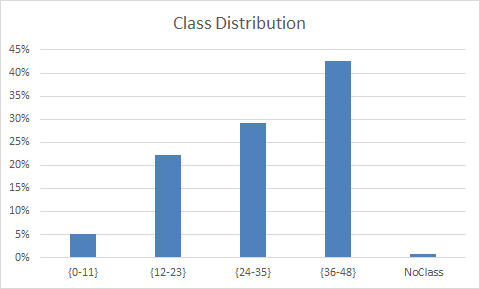
\includegraphics[width=0.49\linewidth]{Figures/class_distribution_als.png}
  	\caption{Class distribution of the ALS dataset.}
  	\label{fig:als_distribution}
  \end{figure}
  
\subsection{Discret ALS Dataset}
\label{subsection:discretals}

Because some of the techniques used cannot be directly applied to numeric data the following discretization was applied on the ALS dataset.

For this discretization some domain knowledge was used to find a discretization that makes more sense than just dividing the feature into $n$ bins. In Tables \ref{table:bp}, \ref{table:pulse}, \ref{table:rr}, \ref{table:percofnormal}, \ref{table:temp}and Figure \ref{fig:weight} the discretization used for the Blood Pressure, Pulse, Respiratory Rate, Percentage of Normal, Temperature and Weight features can be seen, respectively.

For the features where no \hl{decent class } could be found, their values were discretized into $n$ equally sized bins, with $n = 6$. 

\begin{table}[h]
	\begin{center}
		\begin{tabular}{lll}
			\multicolumn{3}{c}{Blood Pressure}                                  \\
			& Systolic          & Diastolic         \\
			Normal                      & \textless 120     & \textless 80      \\
			Pre-Hypertension            & 120-139           & 80-89             \\
			High Blood Pressure Stage 1 & 140-159           & 90-99             \\
			High Blood Pressure Stage 2 & 169-179           & 100-109           \\
			Hypertensive Crysis         & \textgreater= 180 & \textgreater= 110
		\end{tabular}
		\caption{Discretization for both Blood Pressure features.}
		\label{table:bp}
	\end{center}
\end{table}

\begin{table}[h]
	\begin{center}
		\begin{tabular}{ll}
			\multicolumn{2}{c}{Pulse}            \\
			Slow (Bradycardia) & \textless 60    \\
			Resting            & 60-100          \\
			Fast (Tachycardia) & \textgreater100
		\end{tabular}
		\caption{Discretization for the Pulse feature.}
		\label{table:pulse}
	\end{center}
\end{table}
 
\begin{table}[h]
	\begin{center}
		\begin{tabular}{ll}
			\multicolumn{2}{c}{Respiratory Rate} \\
			Slow           & \textless 12        \\
			Normal         & 12-20               \\
			Fast           & 20-24               \\
			Very Fast      & \textgreater24     
		\end{tabular}
		\caption{Discretization for the Respiratory Rate features.}
		\label{table:rr}
	\end{center}
\end{table}

\begin{table}[h]
	\begin{center}
		\begin{tabular}{ll}
			\multicolumn{2}{c}{\% of Normal}              \\
			Very Low Breathing Capacity & \textless50     \\
			Deteriorating               & 50-80           \\
			Normal                      & 80-100          \\
			Athlete                     & \textgreater100
		\end{tabular}
		\caption{Discretization for Percentage of Normal feature.}
		\label{table:percofnormal}
	\end{center}
\end{table}

\begin{table}[h]
	\begin{center}
		\begin{tabular}{ll}
			\multicolumn{2}{c}{Temperature} \\
			Hypothermia  & \textless36.5    \\
			Normal       & 36.5-37.2        \\
			Fever        & \textgreater37.2
		\end{tabular}
		\caption{Discretization for the Temperature feature.}
		\label{table:temp}
	\end{center}
\end{table}

\begin{figure}[h]
   	\centering
   	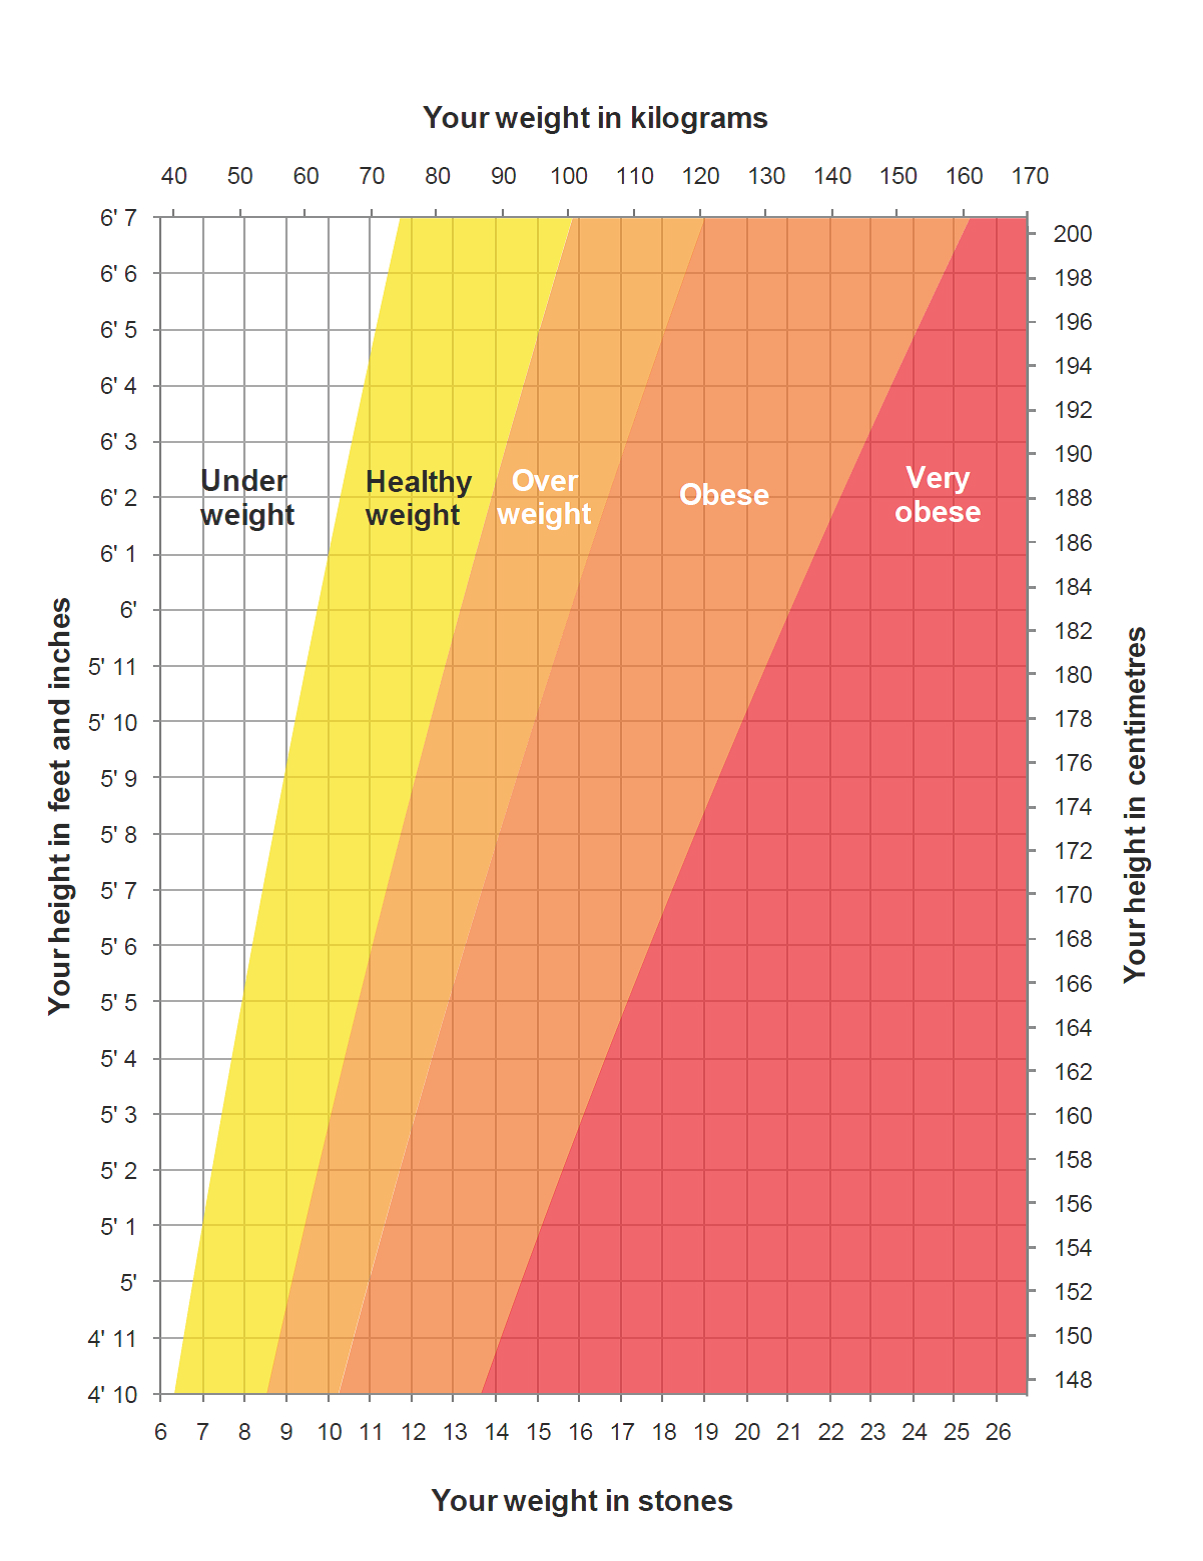
\includegraphics[width=0.49\linewidth]{Figures/adult_weight_height.png}
   	\caption{Discretization for the Weight feature.}
   	\label{fig:weight}
   \end{figure}

\subsection{Hepatitis Dataset}
\label{subsection:hepatitis}

The Hepatitis dataset was made available as part of the ECML/PKDD 2005 Discovery 
Challenge\footnote{http://lisp.vse.cz/challenge/CURRENT/}, it contains data about
 771 patients, and more than 2 million examinations between 1982 and 2001. Based on the work of \cite{Watanabe2003}
 the data was reduced to the most significant exams. In the end 17 variables were used: gender, age, birthdate, birth decade, 
 11 of the most significant exams (GOT, GPT, ZTT, TTT, T-BIL, D-BIL, I-BIL, ALB, CHE, T-CHO and TP) and the results from the
 active biopsies at the time of the exams (type, activity and fibrosis).

Fibrosis is the objective class and it is described by integer values between 0 (no-fibrosis) and 4 (most severe).
 The subset contains 488 patients and the following distribution of 
 classes: 2.05\% of 0, 45.9\% for 1, 21.35\% for 2, 15.19\% for 3 and 15.40\% for 4, as seen in Figure \ref{fig:hep_distribution}.
 
   \begin{figure}[h]
   	\centering
   	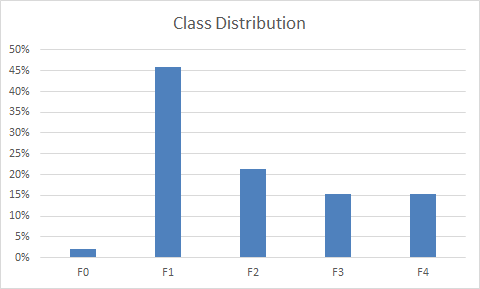
\includegraphics[width=0.49\linewidth]{Figures/class_distribution_hep.png}
   	\caption{Class distribution of the Hepatitis dataset.}
   	\label{fig:hep_distribution}
   \end{figure}

%-------------------------------------------------------------

%\subsection{SEER Dataset}
%\label{subsection:seer}

%The SEER data was requested from the Surveillance, Epidemiology, and End Results (SEER) web site. The data is composed by 9 files where each one contains data related to a specific cancer (breast, colon, urinary, etc.). It is composed by variables that give socio-demographic and cancer specific information concerning an incidence of cancer. Each record represents a particular patient-tumor pair within a registry. Each record is assigned a case number for each patient, and a unique record number for each specific tumor.

 \section{Validation Techniques}
\label{section:validation}

Both of the datasets used describe a disease’s progression, in this case Hepatitis and ALS. 

The reason to use 2 datasets describing different diseases, instead of just one, is to show the generalizability of our approach which hopefully
will show similar results in both.

As previously stated our objective was to focus on finding a way to use the time dimension when performing prognosis, use a patients’ evolution over time, and with that build a generalizable technique whose results would not be so dependent on the data.

For these reasons, and because there are other works where these datasets have been used and preprocessed, \cite{Watanabe2003}, we can base our work on their results, not exploring other pre-processing techniques, and use most of our time on the actual task at hand.

% Please add the following required packages to your document preamble:
% \usepackage[table,xcdraw]{xcolor}
% If you use beamer only pass "xcolor=table" option, i.e. \documentclass[xcolor=table]{beamer}
\begin{table}[h]
		\begin{center}
	\begin{tabular}{l|lll}
		\multicolumn{1}{c|}{\textbf{}}   & \multicolumn{1}{c}{\textbf{+R}}                & \multicolumn{1}{c}{\textbf{-R}}                & \multicolumn{1}{c}{\textbf{}} \\ \hline
		\multicolumn{1}{c|}{\textbf{+P}} & \multicolumn{1}{c}{\cellcolor[HTML]{9AFF99}TP} & \multicolumn{1}{c}{\cellcolor[HTML]{FFCCC9}FP} & \multicolumn{1}{c}{PP}        \\
		\textbf{-P}                      & \cellcolor[HTML]{FFCCC9}FN                     & \cellcolor[HTML]{9AFF99}TN                     & PN                            \\
		& RP                                             & RN                                             & Pop                            
	\end{tabular}
		\caption{Notations in a binary contingency table. Color coding indicates correct (green) and incorrect (pink) rates or counts in the contingency table.}
		\label{tab:notation}
	\end{center}
\end{table}

In Table \ref{tab:notation} we can see notation used. The table is composed by the positive and negative predictions,+P and -P respectively, and the positive and negative real values, +R and -R also respectively. Then TP means the True Positives, TN the number of True Negatives and similarly FP and FN the number of False Positives and False Negatives Respective, respectively. The sum by rows result in PP and PN which are the number of predicted positives and negatives while the sum by columns results in RP and RN, the number of Real Positives and Real Negatives, respectively. The sum of all the real and predicted values gives the size of the population, Pop.

Having the two datasets, the model built and the notation defined the usual evaluation metrics will be used, like \emph{accuracy}, \emph{precision}, \emph{F-measure}\hl{, sensitivity and specificity}.

\emph{Accuracy} is the ratio of correct classifications over all the cases,

\begin{equation}
Accuracy=\frac{TP+TN}{Pop}
\label{eq:accuracy}
\end{equation} 

\emph{Precision}, also called positive predictive value, is the degree to which several measurements provide answers very close to each other. It is an indicator of the scatter in the data.The lesser the scatter, higher the accuracy.

\begin{equation}
Precision= \frac{TP}{PP}
\label{eq:precision}
\end{equation}

\emph{Sensitivity}, also called \emph{true positive rate} or \emph{recall}, is the ability of the model to identify positive cases, in other words this metric shows the overall percentage of correctly identified classifications.

\begin{equation}
Sensitivity= \frac{TP}{TP+FN}
\label{eq:sensitivity}
\end{equation} 

Because only measuring the ability to identify the positive cases is useless (a system that always classified something as positive would have a sensitivity of 1), we also use \emph{specificity}. Similarly, \emph{specificity} measures the ability of the system to identify the negative cases.

\begin{equation}
Specificity= \frac{ TN}{FP+TN}
\label{eq:specificity}
\end{equation}

\emph{F-measure}, also called \emph{F1 Score},is ...... Note that the F-measure effectively references the True Positives to the Arithmetic Mean of Predicted Positives and Real Positives, being a constructed rate normalized to an idealized value.

\begin{equation}
\mathit{F\textnormal{-}measure} = 2 \times \frac{ Precision \times Sensitivity}{Precision + Sensitivity}
\label{eq:fmeasure}
\end{equation}

\hl[red]{Because the use of time is the cornerstone of this work it is also needed to see if it was actually relevant. To do this we will look for the use of temporal patterns in the model created and their relevance in the decision process. I.e. if the model is a decision tree the closer to the root this temporal pattern rules, are the more relevant they are in the decision, and that shows the importance of time in this matter.}

\section{Experimental Results}
\label{section:results}

In this section we will present the experimental results of this case study. We begin by describing the baseline for comparison and then present the performance of our approaches using different techniques.

\hl[red]{This sections begins by presenting the baselines, the diagnosis models, the models that perform prognosis similarly to diagnosis. //
	Then, separating by technique used in the estimation phase (regression, decision tree or HMM), we present the performance of the different approaches compared to the baseline. It is important to note that, per estimation method, we separate the results by phase. This means that firstly we introduce the estimation performance and, after that, the overall prognosis performance using those same estimations. } 

\hl{All The results shown use the \emph{accuracy} metric because it is a universal metric and the \emph{F-measure} metric showed no significant change to the presented results. // We will also show a more in depth analysis of some cases where all the metrics will be taken into account. We will show only some, due to the large number of data and graphs generated by this analysis. }

All tests were ran on an Asus U36SD with an Intel® Core™ i5 2430M/2410M Processor, clocked at 2.40 GHz, 8Gb of Ram and running 64 bit Windows 8.1 Pro.
The Weka toolkit\footnote{http://www.cs.waikato.ac.nz/ml/weka/}, version 3.7.10, was used for the regression and decision tree estimations and classifications. While to perform the HMM estimations, the package HMM \footnote{http://cran.r-project.org/web/packages/HMM/index.html} for the programming language R was used.

\subsection{Diagnosis Model}
\label{subsection:diagnosis}

As a baseline for comparison with the proposed approaches we used two models. \emph{BaselineSingleObservation} is a diagnostic model
 where a single observation in time is used to perform the prognosis. In other words, the state of a patient at instant n is
 used to predict his class at instant $n+1$. On the other hand, \emph{BaselineMultipleObservation} instead of using a single observation,
 uses multiple observations: all information is used here to predict the class at instant $n+1$.

A collection of techniques were used with these models, with both achieving similar results: the accuracy ranged between 40\% and 55\%,
 depending on the dataset, technique and number of time points used, as seen in Figure \ref{fig:baselinesingle} and Figure \ref{fig:baselinemulti}.
 
 \begin{figure}[h]
  \begin{subfigmatrix}{2}
	\subfigure[ALS]{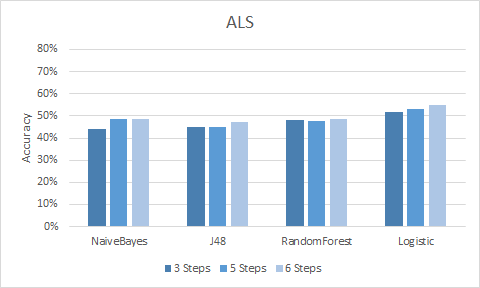
\includegraphics[width=0.49\linewidth]{Figures/base_single_als_tree.png}}
	\subfigure[Hepatitis]{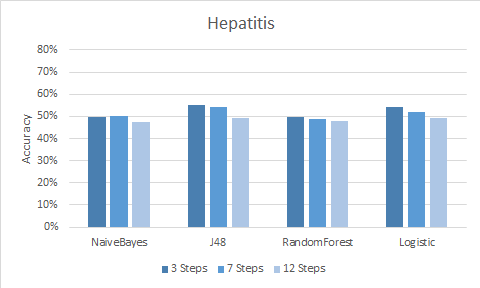
\includegraphics[width=0.49\linewidth]{Figures/base_single_h_tree.png}}
  \end{subfigmatrix}
  \caption{BaselineSingleObs accuracy (several classifiers and number of observations).}
  \label{fig:baselinesingle}
\end{figure}

 \begin{figure}[h]
  \begin{subfigmatrix}{2}
	\subfigure[ALS]{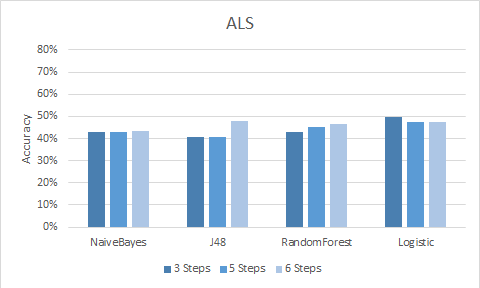
\includegraphics[width=0.49\linewidth]{Figures/base_multi_als_tree.png}}
	\subfigure[Hepatitis]{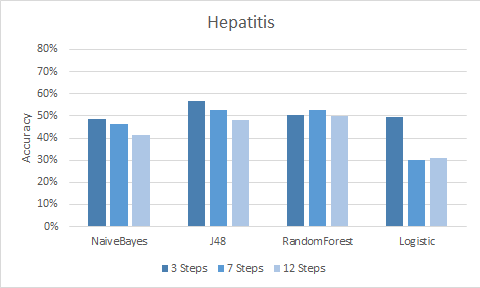
\includegraphics[width=0.49\linewidth]{Figures/base_multi_h_tree.png}}
  \end{subfigmatrix}
  \caption{BaselineMultipleObs accuracy (several classifiers and number of observations).}
  \label{fig:baselinemulti}
\end{figure}

It is interesting to note that the accuracy is almost constant for ALS, for different techniques and number of time steps. However, it is
clear that for Hepatitis those variables are determinant for reaching higher accuracy. The best results tend to be achieved using 3 time steps and 
J48 and Logistic Regression. 

It is also interesting to note that those differences are smoother in the presence of the multiple observations.

\subsection{Regression Techniques}
\label{subsection:regression}

In this section the results of applying regression techniques with out approaches is shown. Because of the different characteristic of the datasets (numeric versus nominal attributes), different regression techniques have been applied in the estimation phase of this work, namely linear regression for the numeric datasets and logistic regression for the nominal.
  
\subsubsection{Estimation Models}
\label{subsubsection:estimation_regression}

As previously mentioned we begin the presentation of our results by analyzing the estimation phase performance.

The results with the univariate and multivariate estimation models for the ALS dataset (numeric) can be seen in 
Figure \ref{fig:estimationals}. These models were built using linear regression as previously said. Both estimation models were 
applied using a different number of observations, $3, 5$ and $6$ time steps.
 Because the dataset is numeric, we evaluated our estimation by the error, the distance, to the actual value at time $t_{n+1}$.
 Both the univariate and the multivariate estimation model presented an average estimation error of around $0.165$, with
 features having errors as high as $0.30$ and as low as $0.01$.
  
\begin{figure}[h]
	\begin{subfigmatrix}{2}
	\subfigure[Univariate Estimation]{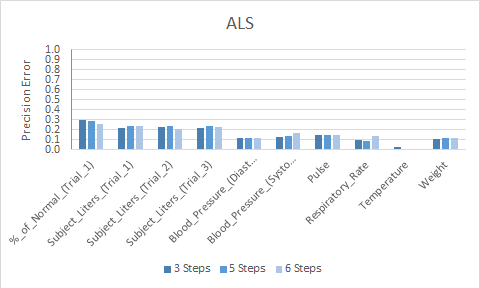
\includegraphics[width=0.49\linewidth]{Figures/estimation_single_als_reg.png}}
	\subfigure[Multivariate Estimation]{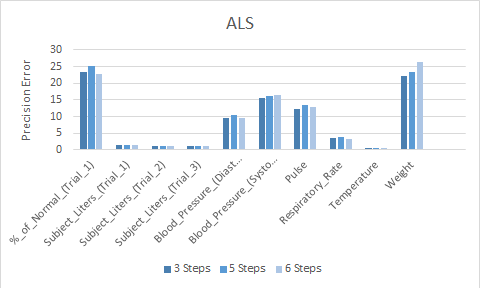
\includegraphics[width=0.49\linewidth]{Figures/estimation_multi_als_reg.png}}
  \end{subfigmatrix}
  \caption{Impact of the number of observations on the accuracy of the linear regression estimation models for each variable, in the ALS dataset.}
  \label{fig:estimationals}
\end{figure}

We can also see in Figure \ref{fig:estimationlogh} the results of using Logistic Regression on the
 Hepatitis dataset. In both cases the average accuracy of estimation rounded the 80\% range, with the multivariate model being consistently
 a bit worse than the model that uses a single variable.
 
 \begin{figure}[h]
	\begin{subfigmatrix}{2}
	\subfigure[Univariate Estimation]{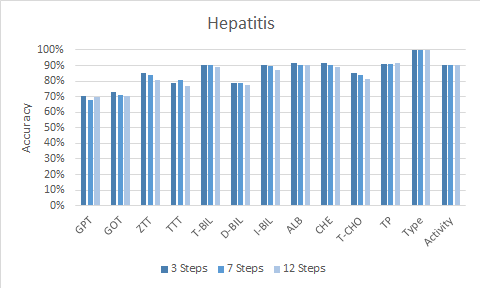
\includegraphics[width=0.49\linewidth]{Figures/estimation_single_h_log.png}}
	\subfigure[Multivariate Estimation]{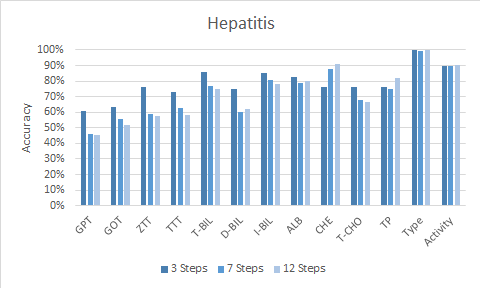
\includegraphics[width=0.49\linewidth]{Figures/estimation_multi_h_log.png}}
  \end{subfigmatrix}
  \caption{Impact of the number of observations on the accuracy of the logistic regression estimation models for each variable, in the hepatitis dataset.}
  \label{fig:estimationlogh}
\end{figure}

\hl{While in the ALS case we cannot descriminate any clear difference between the two estimation models in the Hepatitis dataset, as previously stated, the multivariate approach performed a bit worse than the univariate model. Also in the ALS case we can see a slight trend of improvement in the estimations with the increase of snapshots used, while in the other case the oposite is noteable.}

In Figure \ref{fig:estimationtimelinear} and Figure \ref{fig:estimationtimelog}, we can see the performance analysis, in milliseconds, of the estimation
 phase. It is important to note that no significant difference was noticed between the univariate and multivariate estimations when using linear regression.
 The same cannot be said about logistic regression where the overall estimation of the features on the multivariate
approach took about $(N steps \times 3)$ times more than the univariate.

\begin{figure}[h]
	\begin{subfigmatrix}{2}
		\subfigure[Average Estimation Time]{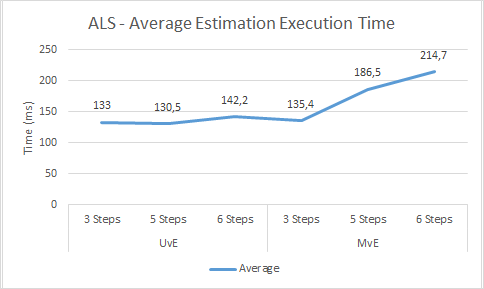
\includegraphics[width=0.49\linewidth]{Figures/time_estimation_average_linear_als.png}}
		\subfigure[Total Estimation Time]{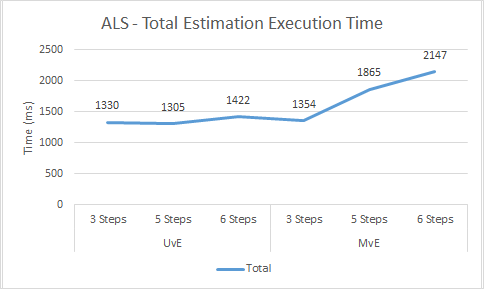
\includegraphics[width=0.49\linewidth]{Figures/time_estimation_total_linear_als.png}}
	\end{subfigmatrix}
	\caption{Execution time of feature estimation in the ALS dataset using Linear Regression.}
	\label{fig:estimationtimelinear}
\end{figure}

\begin{figure}[h]
	\begin{subfigmatrix}{2}
		\subfigure[Average Estimation Time]{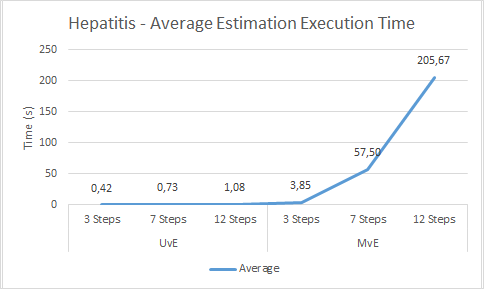
\includegraphics[width=0.49\linewidth]{Figures/time_estimation_average_log_h.png}}
		\subfigure[Total Estimation Time]{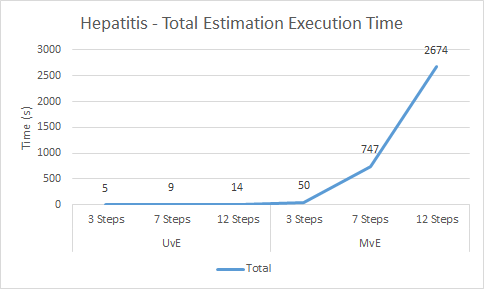
\includegraphics[width=0.49\linewidth]{Figures/time_estimation_total_log_h.png}}
	\end{subfigmatrix}
	\caption{Execution time of feature estimation in the hepatitis dataset using Logistic Regression.}
	\label{fig:estimationtimelog}
\end{figure}

\subsubsection{Prognosis Results}
\label{subsubsection:prognosis_regression}

Finally we will evaluate the performance of the prognosis model, using the estimations presented in the previous section.

The overall prognosis accuracy achieved by using various techniques with our approaches, on the predictions achieved by using regression 
techniques, can be seen in Figure \ref{fig:accuracyregression}. It is observable that decision tree classifiers outperform the other techniques, with
both of them, J48 and RandomForest, achieving better accuracies than the other techniques as well as the corresponding baselines. In the ALS dataset,  J48 and RandomForest were able to improve the results in more than 15\%, with both estimation models. In the Hepatitis dataset the $UvE$ model clearly improved the final accuracy of the prognosis, achieving an improvement of about 20\%. The $MvE$ model didn't do so well only improving the final prognosis by 5\%. 

Figure \ref{fig:impactregression} shows the relation between the number of observations and the final accuracy of the prognosis, using both, $UvE$ and $MvE$ estimation models, and a variety of techniques. It interesting to note that in the ALS dataset and using linear regression we can see distinctly that the number of steps used and the overall accuracy are directly proportional. In the Hepatitis datasets the opposite relation is notable, as the number of time steps used increases the accuracy decreases or maintains. This leads us to think that, in this dataset, the furthest points in time are not as relevant to perform the prognosis as the ones closer to $t_{n+1}$. If this happens because of the nature of the disease or because of the characteristics of the data we are not certain.

 \begin{figure}[h]
  \begin{subfigmatrix}{2}
	\subfigure[ALS - linear regression estimations]{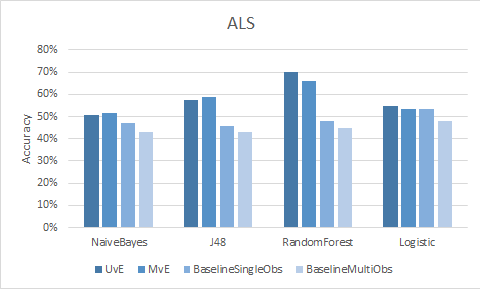
\includegraphics[width=0.49\linewidth]{Figures/accuracy_als_reg.png}}
	\subfigure[Hepatitis - logistic regression estimations]{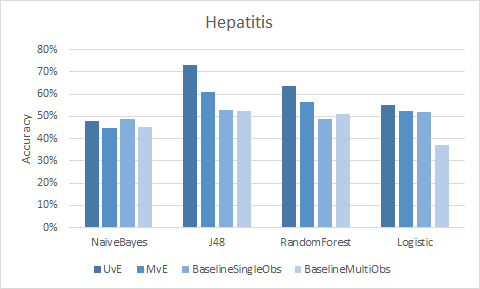
\includegraphics[width=0.49\linewidth]{Figures/accuracy_h_log.png}} %grafico Hepatiti logistic
  \end{subfigmatrix}
  \caption{Accuracy of different models.}
  \label{fig:accuracyregression}
\end{figure}

 \begin{figure}[h]
  \begin{subfigmatrix}{2}
	\subfigure[ALS - linear regression estimations]{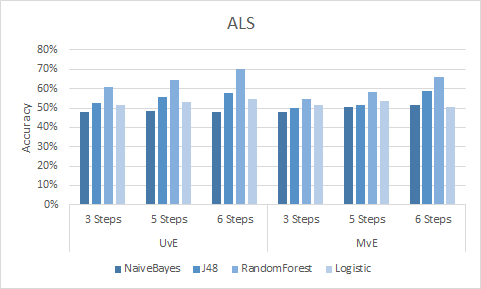
\includegraphics[width=0.49\linewidth]{Figures/impact_als_reg.png}}
	\subfigure[Hepatitis - logistic regression estimations]{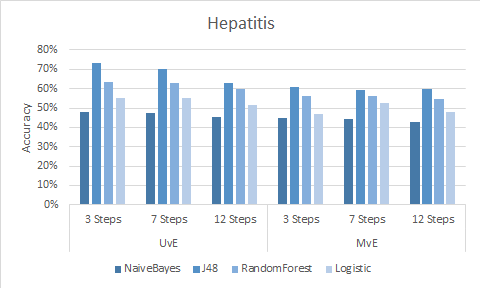
\includegraphics[width=0.49\linewidth]{Figures/impact_h_log.png}} %grafico Hepatiti logistic
  \end{subfigmatrix}
  \caption{Impact of the number of observation on prognosis models.}
  \label{fig:impactregression}
	\end{figure}
	
\hl{In Figure \ref{fig:fmeasureregression} the \emph{F-measure} is show for the different approaches on both datasets.}
	
 \begin{figure}[h]
 	\begin{subfigmatrix}{2}
 		\subfigure[Univariate Estimation - ALS]{\includegraphics[width=0.49\linewidth]{Figures/metrics/als-reg-approach1-fmeasure.png}}
 		\subfigure[Multivariate Estimation - ALS]{\includegraphics[width=0.49\linewidth]{Figures/metrics/als-reg-approach2-fmeasure.png}}
 		\subfigure[Univariate Estimation - Hepatitis]{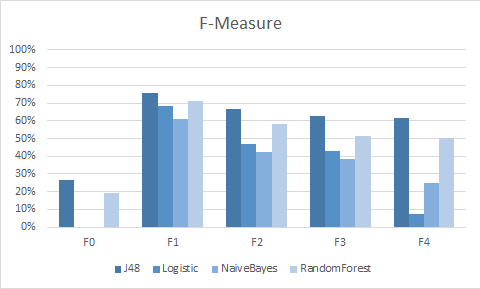
\includegraphics[width=0.49\linewidth]{Figures/metrics/Hepatitis-log-approach1-fmeasure.png}}
 		\subfigure[Multivariate Estimation - Hepatitis]{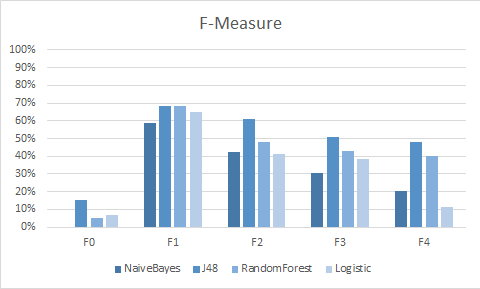
\includegraphics[width=0.49\linewidth]{Figures/metrics/Hepatitis-log-approach2-fmeasure.png}}
 	\end{subfigmatrix}
 	\caption{Different metrics for the overall prognosis using logistic regression on the Hepatitis dataset.}
 	\label{fig:fmeasureregression}
 \end{figure}
	
 \subsection{Decision Tree}
\label{subsection:dt}

In this section, J48 \footnote{http://weka.sourceforge.net/doc.dev/weka/classifiers/trees/J48.html} was used as the estimation technique. J48 is an implementation of Quinlan's C4.5 algorithm \cite{Quinlan1993}. Because J48 cannot handle numeric classification this technique was used on the hepatitis dataset and on the discretized version of the ALS dataset. The results were as follows.

\subsubsection{Estimation Models}
\label{subsubsection:estimation_dt}

Again, before assessing the results of our prognosis approach, we evaluate the impact of the number of observations used, on the 
quality of the estimations made through the two estimation models proposed.

Figure \ref{fig:estimationtreeals} and Figure \ref{fig:estimationtreeh} show the results with univariate and multivariate estimation models. Both estimation models were applied using a different number of observations. 
 
 \begin{figure}[h]
 	\begin{subfigmatrix}{2}
 		\subfigure[Univariate Estimation]{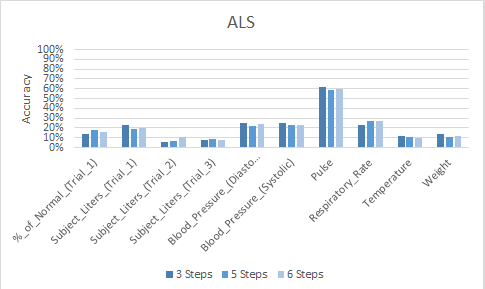
\includegraphics[width=0.49\linewidth]{Figures/estimation_single_als_tree.png}}
 		\subfigure[Multivariate Estimation]{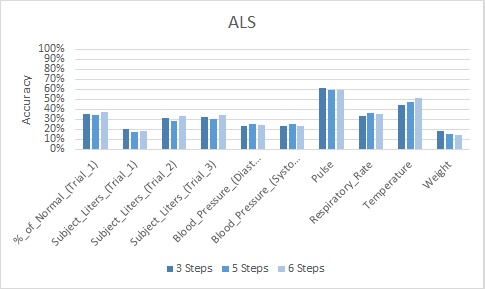
\includegraphics[width=0.49\linewidth]{Figures/estimation_multi_als_tree.png}}
 	\end{subfigmatrix}
 	\caption{Impact of the number of observations on the accuracy of the decision tree estimation models for each variable using both univariate and multivariate models on the discrete ALS dataset.}
 	\label{fig:estimationtreeals}
 \end{figure}
 
\begin{figure}[h]
  \begin{subfigmatrix}{2}
	\subfigure[Univariate Estimation]{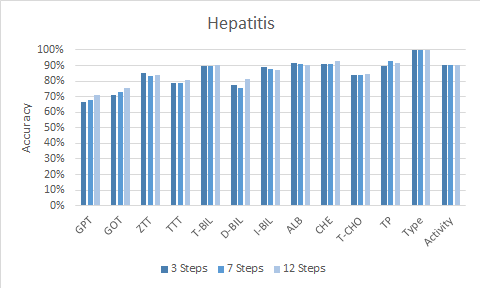
\includegraphics[width=0.49\linewidth]{Figures/estimation_single_h_tree.png}}
	\subfigure[Multivariate Estimation]{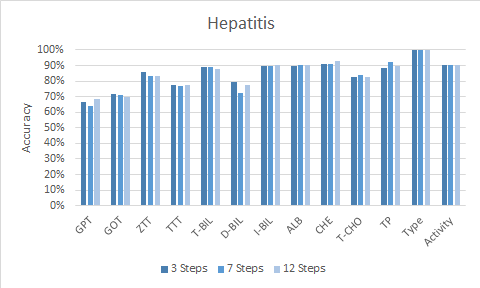
\includegraphics[width=0.49\linewidth]{Figures/estimation_multi_h_tree.png}}
  \end{subfigmatrix}
  \caption{Impact of the number of observations on the accuracy of the decision tree estimation models for each variable using both univariate and multivariate models on the Hepatitis dataset.}
  \label{fig:estimationtreeh}
\end{figure}
 
\hl{The ALS dataset estimations perform very poorly with an average of 21\% and 32\% on the UvE and MvE models, respectively. While the results are poor, there can be noticed a slight improvement by using the multivariate model. This result may be caused by the discretization that was used. }
 
On the Hepatitis dataset both models reach similar levels of accuracy, with quite good results for the majority of the Hepatitis variables
 (above 80\%). It is interesting that there is a slight trend to increase the accuracy as the number of observations get higher.

\hl[red]{Despite our expectations, it seems that there is no improvement on using multivariate-based estimation.}

In Figures \ref{fig:estimationtimetreeals} and \ref{fig:estimationtimetreeh}, the average and total time of execution, in milliseconds, for the feature estimation phase, using J48, is presented.

It is important to note that, on the Hepatitis dataset, even though the estimation using logistic regression had similar results (Figure \ref{fig:estimationlogh}), when looking into to the accuracy of the estimation, it took much longer to estimate the results
 ($3\times$ more in the fastest case and $800\times$ more in the slowest, (Figure \ref{fig:estimationtimelog})).
 
On the ALS case, the time performance was very similar to the linear regression estimation, (see Figure \ref{fig:estimationtimelinear}), with no significant difference worth mentioning.

\begin{figure}[h]
	\begin{subfigmatrix}{2}
		\subfigure[Average Estimation Time]{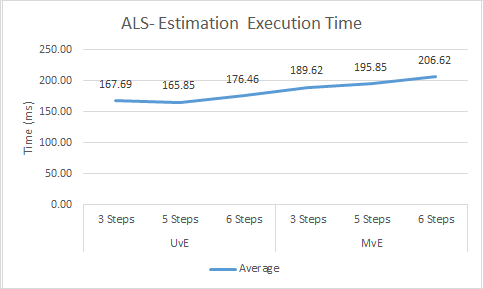
\includegraphics[width=0.49\linewidth]{Figures/time_estimation_average_tree_als.png}}
		\subfigure[Total Estimation Time]{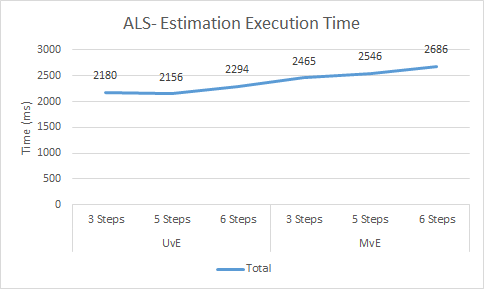
\includegraphics[width=0.49\linewidth]{Figures/time_estimation_total_tree_als.png}}
	\end{subfigmatrix}
	\caption{Execution time of feature estimation in the hepatitis dataset using Decision Trees.}
	\label{fig:estimationtimetreeals}
\end{figure}

\begin{figure}[h]
	\begin{subfigmatrix}{2}
		\subfigure[Average Estimation Time]{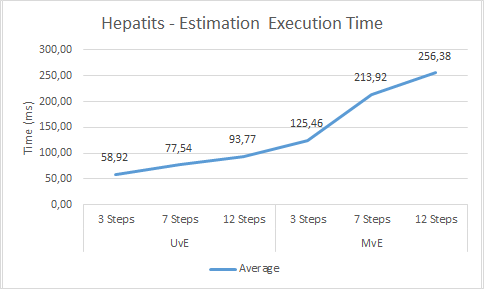
\includegraphics[width=0.49\linewidth]{Figures/time_estimation_average_tree_h.png}}
		\subfigure[Total Estimation Time]{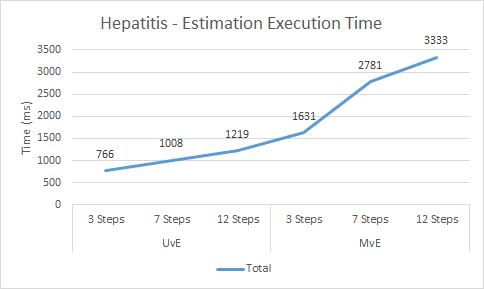
\includegraphics[width=0.49\linewidth]{Figures/time_estimation_total_tree_h.png}}
	\end{subfigmatrix}
	\caption{Execution time of feature estimation in the hepatitis dataset using Decision Trees.}
	\label{fig:estimationtimetreeh}
\end{figure}

\subsubsection{Prognosis Results}
\label{subsubsection:prognosis_dt}

The overall prognosis accuracy achieved by using different techniques on the decision tree estimations can be seen in Figure \ref{fig:accuracytree}.
The improvements on the accuracy of our approach are always present when compared to the ones achieved by baseline models also shown in the same figure. In the Hepatitis dataset the improvements round about 20\%, while in the ALS dataset the improvements are more modest with the UvE model improving around 5\%, with most classification techniques, and achieving similar results as the baseline with the MvE model.

\hl[red]{It is also curious to note that even though the MvE estimations were a little better, the overall prognosis using this estimations was consistently worse its univariate counterpart.}

Figure \ref{fig:impactobservationstree} shows the relation between the number of observations and the final accuracy of the prognosis, using both, UvE and MvE estimation models, and a variety of techniques. Again, and similarly to the regression estimations, it is interesting to note that on the hepatitis case the higher number of observations become prejudicial to the UvE model, which means that the values from the long past do not help to estimate future values. And on the ALS case you can see the inverse relation while much less noticeable than when using linear regression to perform the estimations.

Again there is no clear difference between both estimation models, but decision trees (through C4.5 algorithm – J48 and the RandomForest ensemble) always perform better than the other models. 

 \begin{figure}[h]
 	\begin{subfigmatrix}{2}
 		\subfigure[ALS - accuracy using decision tree estimations]{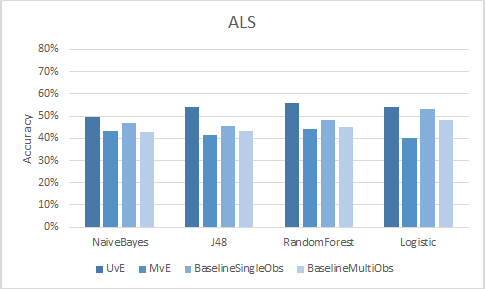
\includegraphics[width=0.49\linewidth]{Figures/accuracy_als_tree.png}}
 		\subfigure[Hepatitis - accuracy using decision tree estimations]{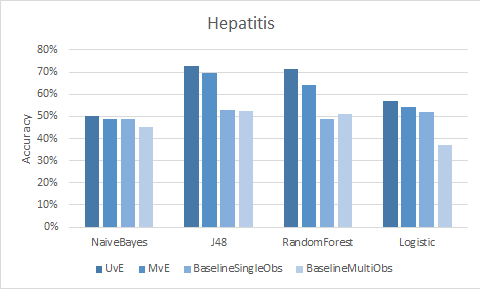
\includegraphics[width=0.49\linewidth]{Figures/accuracy_h_tree.png}}
 	\end{subfigmatrix}
 	\caption{Accuracy of different models using the decision trees estimations.}
 	\label{fig:accuracytree}
 \end{figure}
 
 \begin{figure}[h]
 	\begin{subfigmatrix}{2}
 		\subfigure[ALS - accuracy using decision tree estimations]{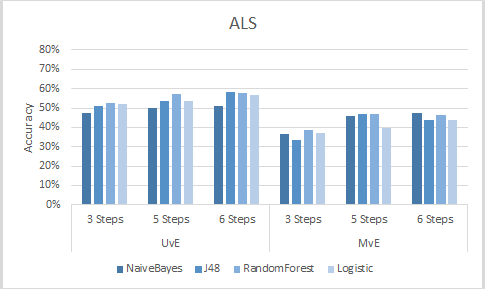
\includegraphics[width=0.49\linewidth]{Figures/impact_als_tree.png}}
 		\subfigure[Hepatitis - accuracy using decision tree estimations]{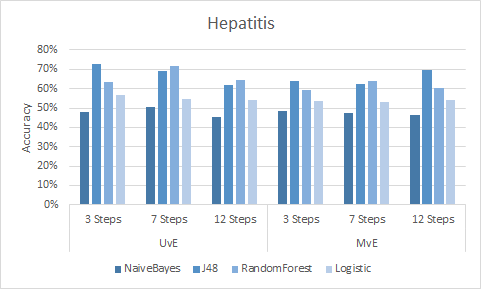
\includegraphics[width=0.49\linewidth]{Figures/impact_h_tree.png}}
 	\end{subfigmatrix}
 	\caption{Impact of the number of observation on prognosis models using the decision trees estimations.}
 	\label{fig:impactobservationstree}
 \end{figure}

\subsection{HMM}
\label{subsection:hmm}

In this final section, HMMs were used in the estimation phase. Because HMMs cannot handle directly numeric classification the same discretization of the ALS dataset was used.

The HMMs we used had one state per time step, so if we had a sequence with data from 7 time instances our HMM 
would have 7 states. All the probability distributions, $\lambda$, would then be initialized randomly and normalized 
so that the probability distribution equals 1.

We would then train one HMM per class, using the Baum-Welch algorithm, which is used to adjust $\lambda$ to maximize the 
likelihood of the training set. The training set was composed by a subset of the data that had the specific class. 

The prediction phase was done by concatenating all the possible classes to the observed sequence and applying the forward
 algorithm with that sequence and the matching class HMM. The forward algorithm calculates the likelihood that the HMM 
 generated the sequence. The sequence with the highest likelihood was chosen and so the concatenated class was the estimation.

\subsubsection{Estimation Models}
\label{subsubsection:estimation_hmm}


Figure \ref{fig:estimationhmmals} shows the results with univariate and multivariate estimation models in the ALS dataset,
 respectively, and Figure \ref{fig:estimationhmmh} shows the same results when applied on the Hepatitis dataset. A different number of time steps were used with each estimation model.

\begin{figure}[h]
 	\begin{subfigmatrix}{2}
 		\subfigure[Univariate Estimation]{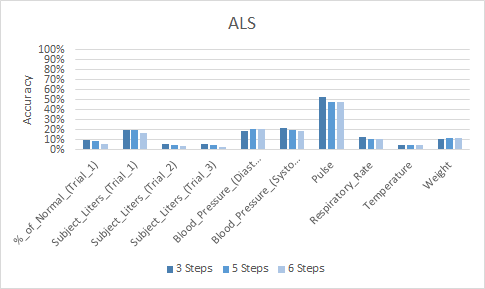
\includegraphics[width=0.49\linewidth]{Figures/estimation_single_als_hmm.png}}
 		\subfigure[Multivariate Estimation]{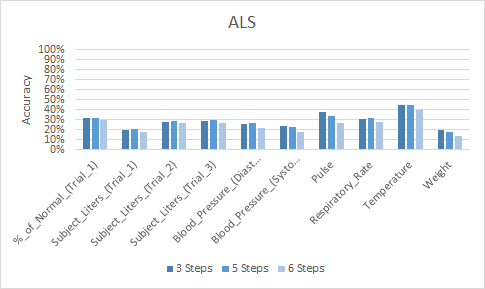
\includegraphics[width=0.49\linewidth]{Figures/estimation_multi_als_hmm.png}}
 	\end{subfigmatrix}
 	\caption{Impact of the number of observations on the accuracy of the HMM estimation models for each variable using both univariate and multivariate models in the ALS dataset.}
 	\label{fig:estimationhmmals}
 \end{figure}
 
\begin{figure}[h]
  \begin{subfigmatrix}{2}
	\subfigure[Univariate Estimation]{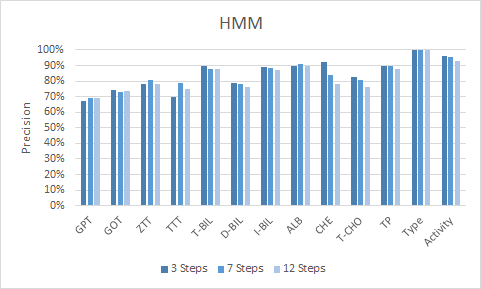
\includegraphics[width=0.49\linewidth]{Figures/estimation_single_h_hmm.png}}
	\subfigure[Multivariate Estimation]{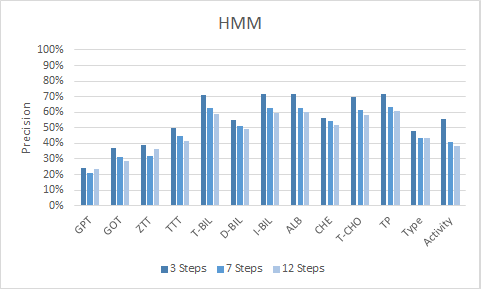
\includegraphics[width=0.49\linewidth]{Figures/estimation_multi_h_hmm.png}}
  \end{subfigmatrix}
  \caption{Impact of the number of observations on the accuracy of the HMM estimation models for each variable using both univariate and multivariate models in the Hepatitis dataset.}
  \label{fig:estimationhmmh}
\end{figure}

\hl{On the ALS case, the average estimation accuracy was of 13\% and 4\%, in the UvE and MvE approaches respectively. This poor performance might be caused by the discretization that was applied to the data. It can also be seen that the number of snapshots used has and inverse relation with the accuracy of the estimations, with the accuracy decreasing with the increase of the number of time steps used.}

\hl{On the other hand, on the hepatitis dataset the average estimation accuracy was of 83\% and 49\%, in the UvE and MvE approaches respectively. This is a very similar results to when using regression of decision trees on the UvE model of this dataset. The MvE performed considerably worse that any other technique used.}

\hl{In Figure \ref{fig:estimationtimehmmals} and \ref{fig:estimationtimehmmh}, we can see the performance analysis, in seconds, of the estimation phase using HMMs. As previously said the Baum-Welch algorithm was used in this step. This algorithm tries to maximize the likelihood of the training set and its result, the model's configuration, is a local maximum. Because of this fact this algorithm is ran X times, X iterations, to try to find the optimum solution. The execution times presented here represent the time taken to run 1 iteration of the algorithm, the estimation results shown, were achieved by performing 50 iterations.}

While in the ALS case, this technique presented a very bad performance. In the Hepatitis case, it achieved similar results in the estimation accuracy, in the $UvE$ approach while the $MvE$ performed significantly worse than any other, (see Figure \ref{fig:estimationlogh} and Figure \ref{fig:estimationtreeh}).
But, in both cases, the time to make those estimations was much longer than any other technique. Even longer than the Logistic regression alternative on the hepatitis dataset, being between $8$ and $200\times$ slower than it and between $100$ and $6880\times$ slower than decision trees (Figure \ref{fig:estimationtimelog} and Figure \ref{fig:estimationtimetreeh}).
 
\hl[red]{TODO - faltam explicaçoes}
 
\begin{figure}[h]
  \begin{subfigmatrix}{2}
	\subfigure[Average Estimation Time]{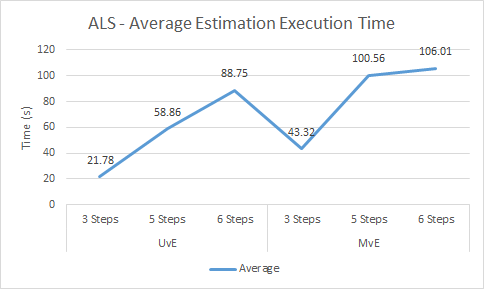
\includegraphics[width=0.49\linewidth]{Figures/time_estimation_average_hmm_als.png}}
	\subfigure[Total Estimation Time]{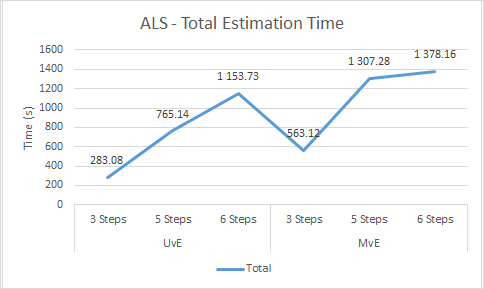
\includegraphics[width=0.49\linewidth]{Figures/time_estimation_total_hmm_als.png}}
  \end{subfigmatrix}
  \caption{Execution time of feature estimation in the ALS dataset using HMMs.}
  \label{fig:estimationtimehmmals}
\end{figure}

\begin{figure}[h]
	\begin{subfigmatrix}{2}
		\subfigure[Average Estimation Time]{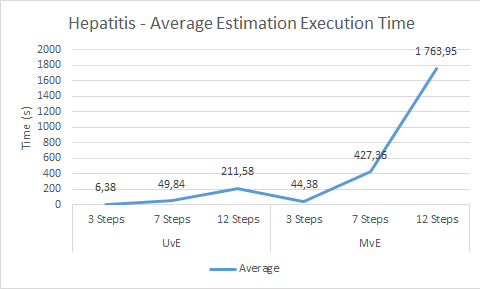
\includegraphics[width=0.49\linewidth]{Figures/time_estimation_average_hmm_h.png}}
		\subfigure[Total Estimation Time]{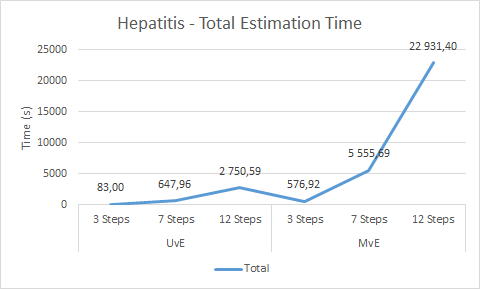
\includegraphics[width=0.49\linewidth]{Figures/time_estimation_total_hmm_h.png}}
	\end{subfigmatrix}
	\caption{Execution time of feature estimation in the hepatitis dataset using HMMs.}
	\label{fig:estimationtimehmmh}
\end{figure}

\subsubsection{Prognosis Results}
\label{subsubsection:prognosis_hmm}

In Figure \ref{fig:accuracyhmm} the accuracy of the various models is shown using different techniques and the HMM estimations.\hl{ In the ALS case, as is was to expect the overall accuracy was the worst found so far, being close to the baseline, but in most cases a bit worse.} In the Hepatitis case it is curious to note that, even though the accuracy of the estimations in the univariate model is very similar, the overall prognosis accuracy is considerably worse. \hl{This might derive from the fact that the correct estimations made with this technique are not as relevant to the final prognosis as the ones made by using decision trees.}

The impact of the amount of time steps, number of observations, used can be seen in Figure \ref{fig:impactobservationshmm}. Here no clear relation can be extracted, with the overall performance not following any pattern in relation with the technique used or the amount of snapshots. 

 \begin{figure}[h]
 	\begin{subfigmatrix}{2}
 		\subfigure[ALS - HMM estimations]{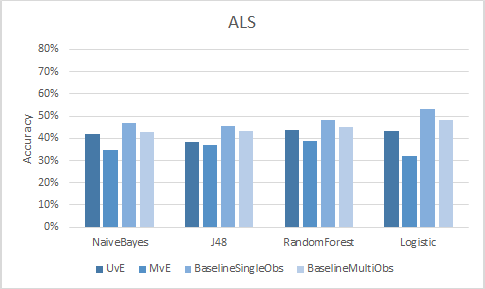
\includegraphics[width=0.49\linewidth]{Figures/accuracy_als_hmm.png}}
 		\subfigure[Hepatitis - HMM estimations]{\includegraphics[width=0.49\linewidth]{Figures/accuracy_h_hmm.png}} %grafico Hepatiti logistic
 	\end{subfigmatrix}
 	\caption{Accuracy of different models using the HMM estimations.}
 	\label{fig:accuracyhmm}
 \end{figure}
 
 \begin{figure}[h]
 	\begin{subfigmatrix}{2}
 		\subfigure[ALS - HMM estimations]{\includegraphics[width=0.49\linewidth]{Figures/impact_als_hmm.png}}
 		\subfigure[Hepatitis - HMM estimations]{\includegraphics[width=0.49\linewidth]{Figures/impact_h_hmm.png}} %grafico Hepatiti logistic
 	\end{subfigmatrix}
 	\caption{Impact of the number of observation on prognosis models using the HMM estimations.}
 	\label{fig:impactobservationshmm}
 \end{figure}

\subsection{Discussion}
\label{subsection:discussion}

Currently, medical practice is helped by a variety of computer-aided tools, dedicated to help physicians taking the most
 appropriate decisions. However, despite the importance of prognosis, it did not deserved dedicated tools, and in the majority 
 of situations, it has been addressed as a simple diagnosis problem, without exploring the temporality involved.

In order to mimic physicians practice, computer-aided prognosis should take into attention patients’ evolution, considering the 
different observations made along time. In this dissertation, we formalize both diagnosis and prognosis problems, making clear the
 differences between them, and propose a method to transform the prognosis into a diagnosis task, based on the composition
 of classification over the estimation of observation values. As described above, what distinguishes this approach, from what 
 is found in the literature, is the use of temporal dependencies of the data in order to estimate the future values of every 
 feature and with those values perform a diagnostic in the future. 
 
 Taking into account the presented results of the techniques used, we can say that HMM were clearly the used method that performed
  the worse. Not only they took a lot longer to perform the estimations but, their results still palled when compared to the use of 
  regressions or decision trees. The other two methods achieved really similar results, when dealing with nominal
  datasets, using decision tree is a better approach when it comes to execution time, while the overall prognosis results are fairly close. 
  
  If dealing with numerical dataset, linear regression managed to achieve an improvement over the baseline. Decision trees also did, achieve an improvement, but a much smaller one and HMMs only managed to achieve similar results to the baseline, or even a bit worse. This two last results though, are largely influenced by the discretization that was applied to the data, and maybe with different a discretization it would the results would be better.
  
  Even though this work focus mostly on the estimation step of the proposed approach, the diagnosis phase still has room for improvement which if done can help improve the final results. One example is the use of more complex techniques and ensembles in the classification, that are known to have better performance than simpler decision trees or regressions.
  
  A curious result that counters what initially was thought when this approaches were planned is the performance of the multivariate approach. This approach was initially thought to be better than the univariate, because of its ability to find and use dependency relations between variables. That was in fact not the case in the datasets used. This might be because the data has too much noise or simply the relations between the used variables does not exist. Either way the univariate approach was consistently better.
 
 
\cleardoublepage
 % file "Thesis_Results.tex"

%%%%%%%%%%%%%%%%%%%%%%%%%%%%%%%%%%%%%%%%%%%%%%%%%%%%%%%%%%%%%%%%%%%%%%%%
%                                                                      %
%     File: Thesis_Conclusions.tex                                     %
%     Tex Master: Thesis.tex                                           %
%                                                                      %
%     Author: Andre C. Marta                                           %
%     Last modified : 21 Jan 2011                                      %
%                                                                      %
%%%%%%%%%%%%%%%%%%%%%%%%%%%%%%%%%%%%%%%%%%%%%%%%%%%%%%%%%%%%%%%%%%%%%%%%

\chapter{Conclusions}
\label{chapter:conclusions}

There is a mismatch in the amount of data available in the field of healthcare and the data that is being used in order to gain knowledge.
 As it was shown in this dissertation, diagnosis and prognosis is a very relevant subject in the area of healthcare and that it has been subject 
 to some work in the past years. This work shows that no novel techniques are being introduced, being the same techniques used consistently throughout the years, and a visible lack of work improving on previous research with predicting models being developed independently. 

We also showed that the problem of prognosis is being tackled in the same way of diagnosis, not using the patients’ evolution over time
 in order to improve the results. 

In order to address this issue, we describe a novel approach that transforms prognosis into a diagnosis problem. This solution has two possible variants for the use of time on improving the results of a prognostic model. An univariate and a multivariate one where dependency relationships can be used to improve the final result.
The method was then evaluated and discussed using two different datasets in order to show its’ generalizability.

In this conclusion, we first highlight the main contributions of this work to the temporal pattern mining field and then discuss some directions for future work.

% ----------------------------------------------------------------------
\section{Achievements}
\label{section:achievements}

From the survey presented the lack of use of temporality in the prognosis problem can clearly be identified. 
Our contribution was the proposal and definition of an extensible method that uses the temporality of the data to improve the prognosis result. It is extensible because a lot different techniques or methods can be used in each step of the approach accordingly to the characteristics of the problem and the data.

This extensibility also introduces a level of generality and domain independence to our method that, based on the problem being tackled, allows us choose the various different techniques and configurations that may suit best the specific case. 


\hl[red]{Generalidade e independencia do dominio}


% ----------------------------------------------------------------------
\section{Future Work}
\label{section:future}

From the experimental comparison of the different approaches, over two distinct datasets (with different data characteristics,
 either from the medical and the data points of view), it is clear an improvement trend when using the temporal informed
 methods proposed. The shallow differences between the results of the estimation models, need to be deeply studied and other
 techniques (like Dynamic Bayesian networks) should be explored to enrich the estimation process. In either cases,
 the temporality of this kind of data should be considered as a core aspect of the prognosis.
 
Another possible variation to tackle the prognosis problem presented in this thesis would be to, instead of using the 
values that result from the estimation phase, like in the current approach, the model that represents the evolutionary trend of that
 feature would be used. Then the final classification would be performed on these models.

\cleardoublepage

 % file "Thesis_Conclusions.tex"

% ----------------------------------------------------------------------
%  Bibliography
% ----------------------------------------------------------------------

% Include all references in .bib file, even non-cited ones...
%\nocite{*} % this should be used carefully because it is not correct!

% Produces the bibliography section when processed by BibTeX
%
% Bibliography style
% > entries ordered alphabetically
%\bibliographystyle{plain}
% > unsorted with entries appearing in the order in which the citations appear.
%\bibliographystyle{unsrt}
% > entries ordered alphabetically, with first names and names of journals and months abbreviated
\bibliographystyle{abbrv}
% > entries ordered alphabetically, with reference markers based on authors' initials and publication year
%\bibliographystyle{alpha}
%
% Replacement bibliography styles provided by 'natbib' package
% (plainnat.bst, abbrvnat.bst, unsrtnat.bst )
% > entries ordered alphabetically
%\bibliographystyle{plainnat}
% > unsorted with entries appearing in the order in which the citations appear.
%\bibliographystyle{unsrtnat}
% > entries ordered alphabetically, with first names and names of journals and months abbreviated
\bibliographystyle{abbrvnat}
% > entries ordered alphabetically, with reference markers based on authors' initials and publication year
%\bibliographystyle{alpha}


% External bibliography database file in the BibTeX format
\cleardoublepage
\bibliography{Thesis_bib_DB} % file "Thesis_bib_DB.bib"
% Add entry in the table of contents as chapter
\addcontentsline{toc}{chapter}{\bibname}
\cleardoublepage

% ----------------------------------------------------------------------
%  Appendix (optional)
% ----------------------------------------------------------------------
%\appendix
%%%%%%%%%%%%%%%%%%%%%%%%%%%%%%%%%%%%%%%%%%%%%%%%%%%%%%%%%%%%%%%%%%%%%%%%%
%                                                                      %
%     File: Thesis_Appendix.tex                                        %
%     Tex Master: Thesis.tex                                           %
%                                                                      %
%     Author: Andre C. Marta                                           %
%     Last modified : 21 Jan 2011                                      %
%                                                                      %
%%%%%%%%%%%%%%%%%%%%%%%%%%%%%%%%%%%%%%%%%%%%%%%%%%%%%%%%%%%%%%%%%%%%%%%%

\chapter{Vector calculus}
\label{chapter:appendixVectors}

In case an appendix if deemed necessary, the document cannot exceed a total of 100 pages...

Some definitions and vector identities are listed in the section below.

% ----------------------------------------------------------------------
\section{Vector identities}
\label{section:vectorIdentities}

\begin{equation}
	\nabla \times \left( \nabla \phi \right) = 0
	\label{eq:cross_nnp}
\end{equation}

\begin{equation}
	\nabla \cdot \left( \nabla \times {\bf u} \right) = 0
	\label{eq:dotCross_nnu}
\end{equation}

\cleardoublepage

 % file "Thesis_Appendix.tex"

% ----------------------------------------------------------------------
\end{document}
% ----------------------------------------------------------------------

